\documentclass[a4paper,12pt]{book}
\usepackage{graphicx}
\usepackage{url}
\usepackage{hyperref}
\usepackage{mdwlist} % list without bullet symbol \{itemize*}
\usepackage{wrapfig} % wrap text around image
\usepackage{csquotes} % for displayquote env

\newlength\mystoreparindent
\newenvironment{leftindent}[0]{
\setlength{\mystoreparindent}{\the\parindent}
\setlength{\parindent}{0pt}
}{
\setlength{\parindent}{\mystoreparindent}
}
\setcounter{tocdepth}{0} % only chapters in ToC
\setcounter{secnumdepth}{0} % no numbering of sections

\title{Contact Book}
\date{\today}
\author{Christoph Pickl}

\usepackage{glossaries}

\makeglossaries

\newglossaryentry{inertia}{name=inertia,description={the "lazyness" of an object, as defined by Newton's first law}}
\newglossaryentry{kinesphere}{name=kinesphere,description={the personal space around us within reaching possibilities of our limbs without changing position}}
\newglossaryentry{kinesthesia}{name=kinesthesia,description={awareness of position and movement}}
\newglossaryentry{momentum}{name=momentum,description={when a physical object is moving with a certain speed}}
\newglossaryentry{negativespace}{name=negative space,description={the empty space which is not occupied by matter which can be "danced in"}}
\newglossaryentry{proprioception}{name=proprioception,description={the ability to sense one's own body position}}
\newglossaryentry{smalldance}{name=small dance,description={tiny, unconscious body reactions/movements to maintain balance/stand upright}}
\newglossaryentry{vector}{name=vector,description={a force with strength and direction, usually visualized as an arrow with a certain length}}



\begin{document}

%\pagenumbering{gobble}
%\pagenumbering{arabic}

\maketitle

\tableofcontents
\vfill
\begin{center}
	\textit{Moving in unity.}\\
	\textit{Guided by the moment.}\\
	\textit{In eternal spirals.}
\end{center}
\vfill
\noindent
\small{Get in contact: \url{https://christophpickl.github.io/contactbook/}}
\newpage


\section{About}

\begin{wrapfigure}{R}{0.3\textwidth}
\centering

\includegraphics[width=0.25\textwidth]{images/about.jpg}
\end{wrapfigure}

This little book is written by me for taking my personal notes in a digital form, so it might be used by beginners, and non-beginners alike, who are interested in getting more acquainted with the theoretical background of the fine art of Contact Improvisation Dance, or CI for short as of now.

Whatever is written here does not claim to hold any absolute, objective truth, but merely is a manifestation of my own personal, subjective opinions. I deliberately choose not to be too much "influenced" by the work of others, and as such did not read many books or any literature of CI. Instead, I am trying to solely rely on a more "innocent" approach and write about my experiences and interpretation of it, which is of course very much colored by me as a person and my (movement) background.

Speaking of my background: It is mainly Japanese (Karate, Aikido) and Chinese Martial Arts (Taijiquan), and as such, my focus lies more on a practical approach, where "form follows function", and less about any aesthetic aspects as many might consider be an essential part of dancing in a more narrow definition. Furthermore, as a bodyworker (Shiatsu Therapy and Neo-Tantrism), I emphasize the importance of the non-verbal communication aspect of movement and touch. Whether we express ourselves in a free form art or the way we interact with others without words.

For me personally, the looks are irrelevant, and "right" is what is pragmatic, meaning efficient in time and space (thinking of physics, anatomy and biomechanics), and as well whatever is in alignment with the principles of CI. Besides those more physical aspects, the psychological aspect should be granted at least half of the attention: The benefit for one's mental health, the ability to get to know oneself and others more deeply, and of course a more philosophical/spiritual path which can also be walked with the help of this deep art.
\chapter{Definition}\label{ch:definition}

\begin{wrapfigure}{R}{0.3\textwidth}
\centering
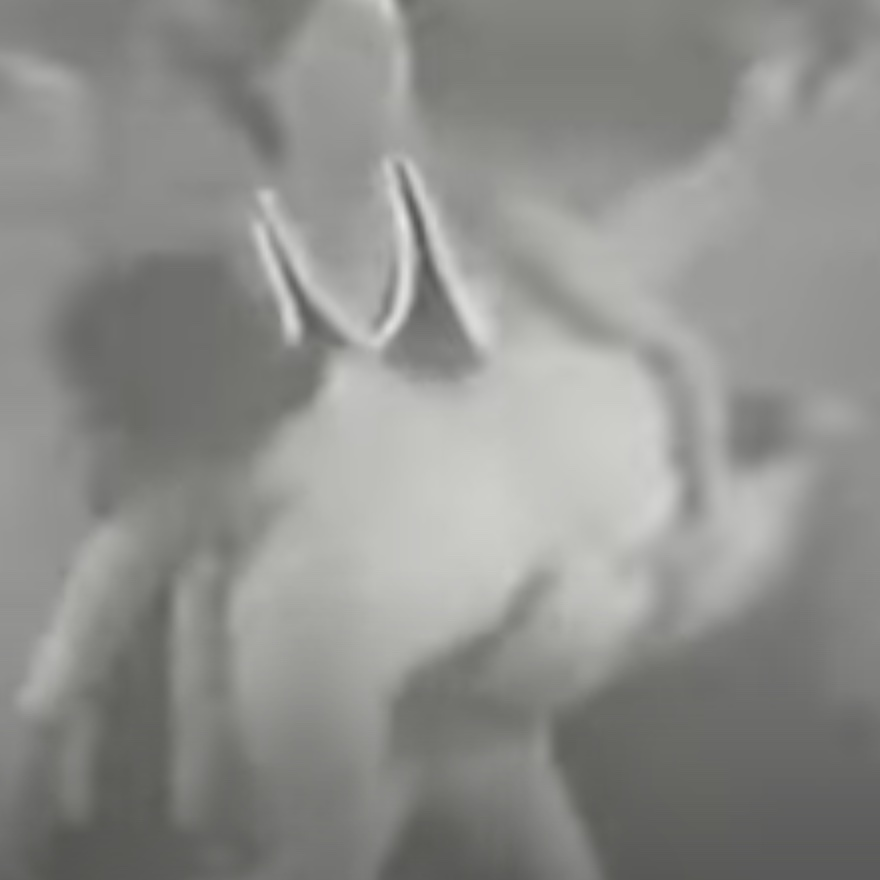
\includegraphics[width=0.25\textwidth]{images/definition}
\end{wrapfigure}

Without a proper definition of what something is, without capturing its \textbf{essence}, it can't be properly talked about.
How does it relate and especially separate itself from other similar systems?
What are its \textbf{goals and principles}, so we can always check whether a specific method or direction is in alignment with these goals and principles.
Not necessarily that it would be wrong, but just to be aware when we step out of our system, and step into something (completely) different.
Communication is usually loaded with \textbf{misunderstandings}, and by having a clear, mutual understanding of what it is we are actually referring to, we can create more \textbf{harmony} in our interaction through clarity (of words).

So what is CI (sometimes also called ``\textit{contact}'' or ``\textit{contact dance}'' in the community) \textbf{compared} to other systems?
A dance, a sport, a (visceral) art-form or post-modern art-sport, partner acrobatics or martial arts?
Well, maybe all of it or none of it, or perhaps depending on how you approach it and what your background is and where you put the emphasis on.
Let's take a look at the different views on it, and by also looking at its history it might get more clear what it is, or what it can be for you.

\section{By Comparison}\label{sec:by-comparison}
%%%%%%%%%%%%%%%%%%%%%%%%%%%%%%%%%%%%%%%%%%%%%%%%%%%%%%%%%%%%%%%%%%%%%%%%%%%%%%%%%%%%%%%%%%%%%%%%%%%%%%%%%%%%%%%%%%%%%%%%

Most of the emphasis is put on the following areas:

\begin{itemize*}
	\item [] \textbf{Experimental dance} -- practice-based research in dance laboratories
	\item [] \textbf{Theatrical form} -- improvised performances and lectures-demonstrations
	\item [] \textbf{Educational tool} -- training for professional dancers in improvisation
	\item [] \textbf{Awareness practice} -- being able to listen to the subtleties in contact
	\item [] \textbf{Social dancing} -- at informal gatherings called ``jams''
\end{itemize*}

At its core it involves \textbf{mindfulness}, sensing and collecting information which requires full presence and attention.
And yes, it is even related to other improvisation practices like improvisation acting: the ``Yes, and \ldots''-concept expressed just physically.

\subsection{Dance}\label{subsec:dance}

It could be considered a form of improvised partner dancing, embedded in contemporary and (post-)modern dance.
Dance improvisation existed already before CI, but it didn't have the \textbf{contact} aspect as CI has, and most of it all the ``\textit{shared point of contact}'' principle.
The development in dance history started with ballet, to modern (Martha Gram, John Cage, Cunningham), and then towards contemporary -- improvisation became not only a research tool, but a performance itself.
Those are mostly vertically, meaning standing, without any floor work involved; whereas in CI, we roll over each other on the floor, something which would be seen as rather unusual in other styles.
We use a \textbf{three-dimensional} spherical space, where every body-part can be a foot -- and be pushed against the ground.

CI is an \textbf{improvised} ``art-form'' (or ``art-sport''), thus without any predefined choreography.
Sometimes CI is used in choreographies, which is then called ``partnering''.
CI is an exploration, a way to try to ``break the system'' as it is improvised.
Nevertheless, CI is not something you would see in the professional dance world, a world where they are walking with very ``nice movements''.

It is not so much that as a CI practitioner, you are serving the \textbf{audience} (in a performance), but rather that the audience is joining you.
It's about getting a visceral reaction from the audience of an improvisation art-form, that they want to join.
Ultimately, there is no difference between dancers and the audience, no hierarchy exists.

It is distinct from other partner dance styles, as those are more focused on the social aspect, whereas CI comes from the art world.
Many other dance forms have also very strict \textbf{gender roles}, where usually the man would lead, and the woman would follow (exceptions exist, like, for example, Lindy Hop, a form of Swing, the mother of Rock'n'Roll).
In CI, everyone dances with everyone, without any clearly defined role.

CI has a strong focus on the \textbf{physical} aspect: How to survive a high-impact volume, which leads to either a crash or a fall?
Lindy Hop has, for example, also some aspects of acrobatics, which Zouk also has a little bit.
Thinking about taking/lifting people on your body, on your core, your center.

There is also a difference in styling, as many \textbf{aesthetically} pleasing dance styles would ``dress to impress''.
In CI, we would typically come wearing our pyjamas (pajamas), sloppy, cozy, comfy, pragmatic.

\subsection{Martial Art}\label{subsec:martial-art}

It is also combined with some minor aspects of eastern philosophy and a few things from the 1960s hippie culture.
The reason being that some founders of CI had their background in the Japanese martial art of \textbf{Aikido}, which is similar to Brazilian Ju-Jitsu.
Gently receiving incoming force and deflect it in circular movements, not resisting but rather listen, perceive, interpret and work with what's there at the moment.

Yet of course CI totally lacks the intention of it being even remotely applied in a contest or let alone in a street fight.
There is no emphasize put on practicality during a physical conflict, still having skills in for example rolling (Judo) can be extremely handy.

\subsection{Applied Physics}\label{subsec:applied-physics}

CI is an exploration of \textbf{physical forces} of one's body in relationship to others by using the principle of sharing weight, touch, and movement awareness, while moving in contact and on the ground.
To play with the artistry of falling unbalanced and counterbalance, with gravity and physics.
To learn the mechanics of the body to handle someone's weight or to be lifted, along with breathing techniques.
Alternatively, it can be stated:

\begin{center}
	``\textit{CI is a three-body-problem with two dancers, being shaped/moved by momentum, gravity, and force, dealing with the third body, the ground/earth.}''
\end{center}

\subsection{Acrobatics}\label{subsec:acrobatics}

The main founder, Steve Paxton himself, was a \textbf{gymnast}, and that might be the reason why still some of CI resembles more partner acrobatics than dancing.
The many (demanding) lifts, and the high velocity and high-impact movements can require a high level of fitness of the practitioners, just like acrobatics does.
Whereas proper partner acrobatics goes way beyond what CI is doing, in terms of physical demands and risky techniques.

\section{Community}\label{sec:community}
%%%%%%%%%%%%%%%%%%%%%%%%%%%%%%%%%%%%%%%%%%%%%%%%%%%%%%%%%%%%%%%%%%%%%%%%%%%%%%%%%%%%%%%%%%%%%%%%%%%%%%%%%%%%%%%%%%%%%%%%

The term ``community'' is in some areas used for people living in the same place, something hippies would do who strive for a more ``natural'' approach to life, people who drop out the system, sharing knowledge about each other, rather than about a specific \textbf{practice}, and helping each other in times of need.
And there is even a current trend in our society that companies are using phrases like ``Come, join the family!'' which even deludes the word family very much.

We use the term ``community'' here for a group of people \textbf{sharing} the same passion for this practice, and getting curious about the other person, from a very basic physical connection.
Sometimes this curiosity goes to their life, experiences, and ideas, which sometimes can lead to afterward also sharing food; from there, friendship can happen.
Sometimes it is also just a great dance partner, but personally, we might have nothing in common, and we also do not want to become friends.
We see each other as ``only dance partners'', and the depth of care we feel is a bit less than, for example, for our beloved neighbor.

In the CI ``community'' this is a bit off though (compared to regular dance scenes), as when someone discontinues to come to classes or jams after a while, we might not be real friends, yet we would still reach out for each other, asking where he is, \textbf{helping} each other out (with health issues, financially) and support if needed.
This happens especially in smaller classes, where there is more of a sense of community.
These silos also happen according to the attitude of the teacher or the jam, where people will converge into specific places; norms will differ based on that.

People who practice or teach CI believe in what they do, in the goodness that it gives the world.
They want to expand the pool to reach more people, and that's why you will see little competition and more \textbf{collaboration} in the scene.
Maybe there will be a bit more competition if it's one's only source of income, a scarce modality; instead of CI being a livelihood, a hobby, a passion.
Some teachers will invite guest teachers, or send their students to another teacher, to a different city, or a teacher who is more technical or in some other way different.
There is not much ``fighting'' among CI practitioners happening, but also collaboration are not so often happening, as it is a very \textbf{individual practice}.
There are festivals, where (abroad) teachers are being invited, but usually when invited, then not by other teachers but by schools, institutions, or organizers.
The norm is nevertheless a ``city-based'' teacher who offers 2--3 classes a week, and sometimes there are ``travelling teachers''.
And there is also a win-win-win in having different student-teacher relationships in one's own workshop.

\section{Stereotype}\label{sec:stereotype}
%%%%%%%%%%%%%%%%%%%%%%%%%%%%%%%%%%%%%%%%%%%%%%%%%%%%%%%%%%%%%%%%%%%%%%%%%%%%%%%%%%%%%%%%%%%%%%%%%%%%%%%%%%%%%%%%%%%%%%%%

There is no clear stereotypical, \textbf{physical appearance} for so-called ``CI people'', as we might have when thinking of people who do Yoga, Hip Hop, or Tantra.
CI practitioners are nevertheless quickly spotted on the dance floor, not so much based on their looks but how they move, how they engage, their behavior with weight.
There appears to be a mutual, unconscious ability to spot each other on the dance floor, which makes them find each other rather quickly -like magic.

A stereotypical CI practitioner is often wearing common \textbf{dance clothes}, nothing too casual or street clothes, but also nothing too fancy.
The age range is rather big, yet for the technical part it's usually around 25--45.
Socioeconomically, it's a little bit on the higher end, meaning people who are \textbf{financially} a bit better off.
Teachers might be willing to give a discount to people who can't easily afford to pay for the classes/workshops, so in case needed, feel free to go ahead and ask, as the worst thing you could get is a ``no'' and in the best case you can afford to go for your dream.
Also, strictly \textbf{religious} people seem not to be attracted by it, most likely because of the touch and the physical proximity.

CI people have no need to attach themselves to a \textbf{subculture} and shape their personality around it; there is no need for ``another stamp'' as is seen so often in other practices.
CI is about the \textbf{physicality}, and less a ``spiritual practice for personal growth'', or a community, as stated above.
Still, the way we move might influence our personality; similar to the increased sensuality when moving Tango, but that's not a big thing in CI\@.
It's very \textbf{egalitarian}, meaning no roles, and a plain physical form.
It's more \textbf{technical}, more raw, and no (moral) values are being conveyed -whereas the egalitarian approach might be a value in itself.
Not only that, but it is \textbf{independent} of sex, gender, age, and body; there is no leading nor following based on sex or gender -just play.
Furthermore, it doesn't convince others of the greatness of CI, although everyone is invited and welcome to join -it's fun.

\section{Jams}\label{sec:jams}
%%%%%%%%%%%%%%%%%%%%%%%%%%%%%%%%%%%%%%%%%%%%%%%%%%%%%%%%%%%%%%%%%%%%%%%%%%%%%%%%%%%%%%%%%%%%%%%%%%%%%%%%%%%%%%%%%%%%%%%%

There is a broad, global community which organizes social dances, so-called ``jams'', regularly, and practitioners often overlap with the Ecstatic Dance \footnote{Many people from Ecstatic Dance often claim to have done ``contact'' but actually have no idea about CI. This confusion is about ``touch-based partner dance'' versus the art-form of CI (sharing weight). These people might also bring in a slight different (sensual-sexual, maybe even Tantric) attitude which is not welcome in CI.} communities.
They are \textbf{social gatherings} without a leader, yet sometimes with someone who facilitates it; similar to jazz jam sessions or Milongas in Tango.
It's an opportunity to practice \textbf{freely}, where people can meet and negotiate together their dance, or observe the practice of their partners.
It's an occasion to meet other fellow practitioners, friends or strangers, old, young, experienced, and novice, and has a bit of a taste of being a hybrid between bodily meditation, psycho-kinesthetic therapy, sports training and a dance improvised session.
They can be regularly in a studio for a few hours, or longer retreat jams for several days in spring resorts where it can be practiced at any hour of the day.

Sometimes you will encounter that the \textbf{facilitator} takes a bit more the lead, by hosting sharing circles at the beginning and/or at the end, and by providing some warm-up exercises.
Sometimes you will have a playlist providing musical background throughout, sometimes you might even encounter a live musician.
Yet, traditionally jams are being kept \textbf{silent}; to let fully unfold of what is alive presently between the dancing partners; to not let the music dictate externally but allow for full expression of what's present, as one of my dance teachers once said: ``\textit{Music makes a dancer stupid}''.

At the end (also sometimes in classes/workshops), you will sometimes find that people engage in an exercise called ``\textbf{round-robin}'', which means that a few couples (or half of the people) are constantly in the center of the room, all the other people sitting on the edge holding space, being present, observing and learning or at least get inspired, giving in their energy, and when you enter/join a couple, another person is leaving, so the number of people stays constant throughout.

\section{Historically}\label{sec:historically}
%%%%%%%%%%%%%%%%%%%%%%%%%%%%%%%%%%%%%%%%%%%%%%%%%%%%%%%%%%%%%%%%%%%%%%%%%%%%%%%%%%%%%%%%%%%%%%%%%%%%%%%%%%%%%%%%%%%%%%%%

In the early beginnings, in the 1970s, every time the founding members practiced CI, they would redefine it, asking the very same question over and over again: ``What is CI \textit{now}?'' An early definition by \textbf{Steve Paxton} and others was (source: CQ Vol. 5:1, Fall 1979):

\begin{displayquote}
``A continuously evolving system of improvised movement.
Two bodies, communicating with each other in physical contact, creating a relationship with the physical laws (motion, gravity, momentum, inertia).
Sensitive, thus relaxed of unnecessary muscular tension, and willing to experience a natural flow.
Techniques may include: Rolling, falling, being upside-down, following, supporting and giving weight.

A physical dialogue ranging from stillness to highly energetic exchange.
Alert enough to stay in an energetic state of physical disorientation, trusting your survival instincts.
A free play seeking for balanced movements, leading to a physical and emotional truth, shared currently, leaving you informed, centered, and enlivened.''
\end{displayquote}

\section{Possible Definitions}\label{sec:possible-definitions}
%%%%%%%%%%%%%%%%%%%%%%%%%%%%%%%%%%%%%%%%%%%%%%%%%%%%%%%%%%%%%%%%%%%%%%%%%%%%%%%%%%%%%%%%%%%%%%%%%%%%%%%%%%%%%%%%%%%%%%%%

Definitions, and the same with any terminology, are time-, space- and person-dependent.
Just as with the improvised nature of CI, it is a constantly moving target.
By asking the same question a week later, the answer you receive will already be different.

There is still a rough \textbf{body of agreement} -- a congruent understanding -- of what it is, and what it is not, leading to a definition stable across time, space, and practitioner.
It's like a tree: The trunk which are the agreed principles, and it's branches and leaves (the styles/adaptations) representing the edges where you can play freely.

\textbf{Steve Paxton} himself stated in 1979:
\begin{displayquote}
	``The exigencies\footnote{exigency = A pressing or urgent situation/requirement/need.} of the form dictate a mode of movement which is relaxed, constantly aware and prepared, and on flowing.
	As a basic focus, the dancers remain in physical touch, mutually supportive and innovative, meditating upon the physical laws relating to their masses: gravity, momentum, inertia, and friction.
	They do not strive to achieve results, but rather, to meet the constantly changing physical reality with appropriate placement and energy.''
\end{displayquote}

\textbf{Nancy Start Smith} once mentioned:
\begin{displayquote}
	``It resembles other familiar duet forms, such as the embrace, wrestling, surfing, martial arts, and the Jitterbug (Lindy Hop and swing dances), encompassing a wide range of movement from stillness to highly athletic.''
\end{displayquote}

\textbf{Daniel Lepkoff} states about the core of CI:
\begin{displayquote}
	``To put focus on bodily awareness and physical reflexes, rather than consciously controlled movements.
	Precedence of body experience first, and mindful cognition second, is an essential distinction between CI and other approaches to dance.''
\end{displayquote}

\textbf{Ray Chung} once announced in a workshop 2009 that:
\begin{displayquote}
	CI is an open-ended exploration of the kinesthetic possibilities of bodies moving through contact.
	Sometimes wild and athletic, sometimes quiet and meditative, it is a form open to all bodies and inquiring minds.
\end{displayquote}

\section{Beyond CI}\label{sec:beyond-ci}
%%%%%%%%%%%%%%%%%%%%%%%%%%%%%%%%%%%%%%%%%%%%%%%%%%%%%%%%%%%%%%%%%%%%%%%%%%%%%%%%%%%%%%%%%%%%%%%%%%%%%%%%%%%%%%%%%%%%%%%%

CI is for sure not a pure \textbf{martial art}, as it has no claim to have any practical fighting application.
Nor is it a competitive \textbf{sport} in any way, as there are no competitions and due to its artistic nature it would be difficult, or at least without much meaning, to judge one as being better than the other.
It has many aspects of partner \textbf{acrobatics}, but lacks many technical possibilities due to the nature of its principles.

It is also not really your regular \textbf{dance} form like Salsa or Tango, due to several reasons: We don't dress (nor dance) to impress but rather show up with our authentic selves; we don't move to only look good or aesthetically (to others); we focus more on the internal and interpersonal aspects than the external ones; we often dance without music; there are no real techniques which can be learned but only guiding principles from which some specific movements can emerge.

As it is the case with so many (or maybe even all?) disciplines: Once the rule has been understood, and you know what you are doing, it can be broken by the student, thus \textbf{becoming a master} of it.
Finally, it has to be mentioned that a system\footnote{In this case we talk about CI as a system, but the forementioned wisdome can be applied to our world's system, politically or economically, to technology, to our endless todo lists \ldots} is supposed to be of service to the user (not the other way round), and its boundaries and dogma should not limit but enrich the applicant.
Whenever the purpose is hindered by the system, the system shall be left behind, and we should remember the original goal which was there in the first place, and not to serve the gods we created.

\section{Beginning}\label{sec:beginning}

As a beginner it is sometimes a bit difficult to get the information to decide whether this art can be something for you or not.
Furthermore, we need to find some information to see what it is, and whether it actually fits us -in our needs but also in regard to the physical requirements on the body.
How to find a school, how to find a teacher, and what to look out for when doing so.
This section should provide you with some directions on doing your first steps into the world of CI.

\subsection{Where to begin?}\label{subsec:where-to-begin?}

To start it's always nice to check some YouTube videos (see the Resources chapter), but please don't be intimidated right away from what you are seeing.
The people you will see on those videos are usually already on a very high level, and that's not what you are going to encounter at first.

Join a recommended teacher and go first to some classes (see ``How to spot a good teacher'' further below).
It is not recommended to immediately go to jams; only after 10-20 classes, to have the basic principles embodied.
And don't give up if your very first experience seems bad; maybe you want to just try another class or another teacher.
Be also aware that CI is not only physical, thus ask yourself: Why and what are you doing?
This will be very beneficial and inspiring for your first steps with CI.

\subsection{Requirements}\label{subsec:requirements}

You might ask yourself for whom is CI fitted?
For whom is it, or is it not a good idea to join?
Are whether there are any physical requirements and how to deal with if one feels a bit touch-averse towards strangers.

In general, it can be said that every body is welcome, but not necessarily every behaviour though.
It is not about age, as even people 70 plus can join, neither about body ability.
Yet some techniques might not be possible to do, or would need some adaption.
Once a student with 72 years would even be able to do shoulder lifts, and he was doing it for many years.
Some of the more crazy things, he mentioned, was better to keep for ``the next life''.

Sharing weight, being in contact with another body, exploring what's happening, where the weight is, the unconscious reaction to balance, \ldots this, anybody can do.
Even with a partially disabled body, with some physical disability like people in a wheelchair can do it, together with physically fit people.
Or also blind people, as they are often also super in tune with weight and different other aspects.
It leads to a very different and interesting kind of exploration, and requires us to renegotiate, to re-explore what kind of communication we can play with.

Even with a huge weight difference, we just need to be more careful about which kinds of lifts to do, and who is carrying whom how.
We need to negotiate what's possible, and sometimes this means no shoulder lifts, and/or no rolling over.
Always respect the abilities of the dance and both bodies by checking each other out, slowly (!) and step-by-step, then it becomes \textit{safer}, yet not necessarily safe!
When about to engage in more advanced (crazy, dangerous) techniques, always do it with a lot of care and a \gls{guardianangel} who will spot you.

In theory, in an ideal world, everyone is welcome, yet it is not advised for people with severe touch aversion to jump into CI, as a solution to their trauma in that field.
It is recommended to better ``tippie toe'' in different kind of forms, and only then see if they want to continue with CI.
Mental challenges sometimes make people join only one (or even half a) class, or sometimes the teacher might even have doubts and expresses that.
People who take too many risks (the ``dangerous ones''), which are throwing themselves on unknown partners, won't be denied access to classes or jams, but dancers will most likely keep their distance to them, as it won't feel safe.

\subsection{How to spot a good teacher}\label{subsec:how-to-spot-a-good-teacher}

There are three realms to consider:

\begin{enumerate}
    \item The \textbf{physical} aspect: The teacher knows what he is teaching, and also being honest about his limitations in that knowledge; or in short: humbleness.
    \item The \textbf{psychological} aspect: This includes the ability to hold space, in case when processes might happen.
    Further, safety is created by the nature of his intention: Does he want to inflate his ego, making himself bigger?
    Does he claim to have a status of a master or guru, or is he ``one of us'' and going for a drink with the students, taking off his teacher's hat.
    Does he want to gain something from you outside the class, besides monetary compensation in a formally agreed transaction?
    \item The \textbf{spiritual} aspect: Watch out for the presence of competition.
    Does he genuinely want the student to be as good or even better as himself?
    Basically, does he have a pure intention to teach, sharing his knowledge (whereas this sharing is also always happening two-way though).
\end{enumerate}

\subsection{Becoming Good}\label{subsec:becoming-good}

What makes a good CI practitioner good can be answered in many ways.
It is for sure not only the obviously physical aspect, but also having the right intention for the dance, a proper attitude and mindset which is led by curiosity, the antidote to being judgmental.
An advanced practitioner is really happy exploring the smallest thing, being able to keep a beginner's mind open, and they know what they know, and they especially also know what they don't know.

For many, dancing with total beginners and total advanced is most enjoyable as they reminder us, showing us the different aspects of the dance.
Both of them are usually very happy to dance with each other as well.
On the other hand, intermediates are usually not happy to dance with beginners, they prefer to only stay with their own level or higher.
They are also usually the ``dangerous ones'', as they know the pathways and the tricks, the form and the looks, but they don't know what they don't know.
They are lacking the listening ability, if something happens which was not predicted in their pathways, like quick changes, they don't know how to handle that.
They also often go faster than their level of attention, and especially very often go faster than their beginner-partner's level of attention.
Having that said: Always respect what your body is able to do, in regard to level, age, and constitution.

A very important tool one should have is also the ability to listen to small/subtle sensations in the body, the change of movement and weight.
An increased awareness of incoming information, inside as well as outside the body via the peripheral nervous system, the so-called \gls{skinesphere}.
It leads us to be able to detect what's going on, thus becoming ``well-informed'' and leading us to become a much better dancer.

More general speaking, which applies to any form or practice:

\begin{itemize}
    \item \textbf{Kindness}: Smile, be gentle and soft.
    \item \textbf{Humbleness}: By not showing off how many years you are doing this-or-that, and not arrogantly teaching beginners.
    \item \textbf{Patience}: Let beginners do their own mistakes, and thus gain their own experience.
\end{itemize}

Everybody learns and everybody teaches.
There are no certificates.
If you have a lot of knowledge, you will share that by your dancing.

Years of practice itself are not necessarily a guarantee for expertise or even mastery!
Some people get stuck at a certain level even after many, many years.
Even lots of experience itself doesn't mean your level of technical practise is going forward.
Even if someone is technical level very advanced: The moment where one stops posing questions, is where one stops developing.
Always keep a beginner's mind: Keep on doing the very same thing, like lifts and spirals, yet stay with curiosity and explore deeper, like the small things and changes, where to focus now, to put your attention and intention to.

\section{Motivation}\label{sec:motivation}

\begin{wrapfigure}{R}{0.3\textwidth}
    \centering
    
\includegraphics[width=0.25\textwidth]{images/motivation}
\end{wrapfigure}

``\textit{If meditation is the process of being in the present moment, in the so-called here-and-now, then Contact Improvisation is the highest form of meditation.}''

Besides for the obvious reason for dancers to expand their skill-set, non-professionals are most likely to start with CI for either simply pleasure of doing it (as it is fun), or even for personal development purposes.
We all come to doing the same things sometimes for very different reasons, and all of them are valid, and some of them might be suboptimal as other methods might be more effective in attaining one's goal.
This section might get you inspired to start, or even motivate you further to deepen and dedicate more of your life into this ``useful'' art.

\subsection{The Power of Touch}\label{subsec:the-power-of-touch}

The tactile experience is most prominent during practicing CI. To be specific, it's the activation of nerve fibers in the skin, so called C-tactile afferents, through gentle and slow stroking with body-like temperature (``warm touch'' leads to release of serotonin, a hormone which makes us feel happy, regulates our emotions and associated with sympathy and interpersonal affection; ``cold touch'' is experienced when being socially excluded, as the skin temperature decreases).
This increases activity in the insular brain region, which is responsible for interoception (perception of the current body state and facilitation of the sense of self).
Through this touch, which can be soft to slide, or deep to the bones, is used to establish a nonverbal, two-way dialogue process, a form of communication.
In the UK alone, about 54\% (among 40,000 participants) want more touch in their lives!
We live in a low-touch society, and mistrusting strangers became a default.

This touch reduces stress (lowered cortisol levels, which is a biomarker for stress-related diseases), increases oxytocin levels (attachment, connectedness) and lower blood pressure.
If a person lacks touch, disorders like depression, a distorted body image, low self-esteem and heightened aggression and self-injurious behavior might occur.
It counteracts a feeling of loneliness and isolation, which is the case in many forms of mental disorders.
Touch releases endogenous opioids, which make us feel relaxed, good, and more resilient.

Yet, touch needs to happen with consent in order to be experienced as something positive.
To want to touch, and want to be touched.
Respecting each other's boundaries, and the possibility to step out of touch at any given moment.
A good CI facilitator will address those things, by, for example, introducing ``no'' exercises, and safety rules at an event.
Especially beginners, who are easily overwhelmed by touch and lust trust in others due to previous bad experiences can benefit from a gender-based group and sharing circles in a safe space to reflect upon.

\subsection{Psychological Benefits}\label{subsec:psychological-health-benefits}

It is said to have positive effects on stress relief, relaxation, well-being, happiness, joy, connectedness, empowerment and feeling more fearless.
Also, a clearer experience of a ``sense of self'' and the body;
being aware of one's own existence.

The massage effect of ``sharing weight'' seems beneficial against anxiety, depression, ADHD, eating disorders (better sense of one's own body), autoimmune diseases, chronic fatigue syndrome, and more.
It also helps with the activation of the parasympathetic nervous system (``\textit{rest and digest}'').

As the attention is attracted to the ``shared zones of contact'', it brings us to the present moment, and thus becomes a mindfulness practice, distracting us from stressful thoughts.
There is no intention to reach a certain goal, but simply exploring movement and touch itself.
This requires us to be attentive, aware and present.

For sure there are benefits in the area of personal and social growth.
Maybe even it could be considered a philosophical, mental, spiritual practice.
Its slowness resembling some meditative state and its fastness to stay in the flow, in the zone, in order to ``survive''.
Like ballet, where dancers stay in the zone of awareness, a meditative state, by doing for example a pliee for more than 15 minutes.
Just in CI, instead of pliees, we do the \gls{smalldance}.

Finally, the personality gets strengthened, by being more aware of one's own needs, and distinguish oneself from the others.
Patterns can be broken, and a positive impact in resilience-building might occur.

\subsection{Social Bonding}\label{subsec:social-bonding}

CI helps us to relate better to others, to create strong social connections, to connect to other people and bodies.
At the beginning, this connection with others might not be so present, as we focus on the technicalities (the bodies, not the peoples); the focus resides on creating a piece, not a community.
The experience of giving and receiving support via ``sharing weight'' for example.
The sensation goes beyond the pure physically into the psychological/emotional realm.
To trust each other, to feel safe again.
Presenting our vulnerabilities and instabilities, ultimately leading to a state of safe intimacy.

Reported experiences during a dance can be: playfulness, surprises, curiosity, flow state, feeling free, being alive; vitality, nourished, energized; connectedness; trust, closeness, deep communication, safe, secure.
The sensation of connectedness feels like being one new, ``third entity'', as it is not clear who gave the impulse to move in a certain way (quote Paxton).
By feeling the other person more, I feel my own boundaries better, thus I feel myself more, ``feeling more home in my own body''.
Yet, negative sensations might occur as well of course, like: boredom, insecurities, doubts, exhaustion, strenuous and being at one's own mercy.

It can connect people from all background, as we all have the same body (being equalized), moving in space, independent of age/gender/sex/belief/religion/color.

\subsection{Soft Skills}\label{subsec:soft-skills}

Through the practice of CI, many soft skills are also trained and enhanced, such as: teamwork, problem-solving, communication, interpersonal skills, adaptability, dependability, and creative thinking; which are all not only important in our personal, but also in our work life.

In \textbf{teamwork}, we achieve a common goal while supporting the strengths of others.
While we dance with a partner, we are looking and seeing where all the other couples are and moving through and around them.
Our goal is to have an enjoyable dance while letting others have one too;
by literally supporting our partner, and choosing together how to navigate the space, we form a small team.
The so-called ``big space'', the heightened awareness of all the people within a room/a jam, we all pay attention to each other, forming a big team.

Every contact is a little kinetic puzzle which requires \textbf{problem-solving} skills.
Like watching two improvisation actors saying ``yes and'' a little too often, and you wonder how they will get out of that; yet with CI the very same happens just physically.
Navigating through space, while watching not to bump into others or hit the wall, and all of that while maybe your partner is trying to balance on your body; all at the same time need to be somehow solved at the moment.

Good \textbf{communication} skills require deep, active listening;
yet with CI we mostly stay in silence, so the attentive listening happens only non-verbally with the whole body.
There is never an agenda, a script, a predefined choreography;
no one knows upfront what's going to happen, who is going to initiate what; yet surprising as it sounds, with good enough listening skills, there will always be clearly communicated what will happen next; by simply listening and responding.

\textbf{Empathy} is an essential part of interpersonal skills, which is practiced in CI by ``feeling the earth through our partner's feet''.
Although you might not know anything about your current dance partner, through this interaction you will experience so much about how they live in this world -bodies speak beyond words.
It's not only physical characteristics like size or weight, but also preferred, applied techniques and general movement choices.
Through this, we might not be aware of facts like country of origin or the family status, but on a different dimension.

There is such a vast variety in contact improvisation dancers that \textbf{adaptability} becomes actually a very common skill which gets acquired very fast due to its necessity.
Obviously the amount of weight one can share with the partner needs to be adjusted;
the differences in height make certain techniques (lifts) maybe more or less easy, or even impossible; and of course the level of experience with body practices in general and CI specifically requires one to adapt to what's there - and possible - at the moment.

A fun contradiction in CI is, that on the one hand you have to be able to completely rely on your partner, building up trust (\textbf{dependability}), and on the other hand to always stay within your own center, being able to catch yourself at any given moment (\textbf{self-reliance}).
Always take care of yourself, while being hyper aware of where your partner is, how he is moving and where he is going;
and also knowing what the other people are doing in the room, having one's awareness spread throughout the space.
Bear also in mind that you can't know what's going to happen, predictions are impossible due to the improvisation nature of CI; thus the name.

Lastly, you will also gain some more insights into yourself, knowing more about your personal boundaries and tolerance for risk.
How we want to be treated, and how to be heard;
our tendency about taking over a conversation; realizing that we are not as heavy as we imagine ourselves to be.
We learn to be vulnerable and to trust others with our vulnerability (``\textit{When I fall, will you catch me?}'').

\subsection{Other Motivations}\label{subsec:other-motivations}

The following subsection contain some reasons which are not the main reason, the main intention, yet are also co-existing.

As a \textbf{body-oriented practice}, it will connect you more to the body, and less to the mind.
In case you are not there (in the moment with full presence), the flow will tell you by bumping and falling.

A very pleasant side effect is that it can also act as a form of \textbf{workout}.
By this, we avoid having to go to the gym and have much more fun in the studio playing with each other.
``\textit{Some people lift weights, we lift bodies}'';
some people run to lose weight, we go dancing.

Because it sparkles \textbf{curiosity} in us, to explore the exercises further.
For some it is a starting point of such exploration, whereas less than half stay with CI, others continue somewhere else.
The love for the capacity to move in a different and new way.
These new pathways are often explored due to its improvised nature, it being part of the dance improvisation world, without any choreography, which often leads to the loss of "why we are doing it", the reason, and simply following someone else's idea.

On a much deeper level it is also a way to ``handle life'', in a nice, safe environment.
A place to see humanity, or better: animality.
In a good kind of way, a monkey kind of way, which is very much fun.

\section{History}\label{sec:history}

\begin{wrapfigure}{R}{0.3\textwidth}
\centering
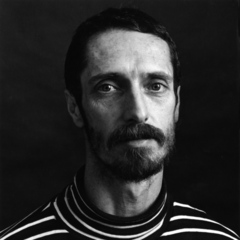
\includegraphics[width=0.25\textwidth]{images/history}
\end{wrapfigure}

In order to know who you are today, I need to know your past, and maybe can even partially predict something about your future.
This applies not only to individuals, but as well to humanity as a whole and localized phenomena like the art of CI itself.
By knowing its origins, we can prevent from diverting too far from it, and reach a deeper understanding of why things the way they are.
And also of course to bring in some kind of attitude of honor, paying our respect to the founding fathers (and mothers).
To bring in some tradition, something our society these days so much lacks and yet so much is in need of (even though it might not be aware of it).

\subsection{Founding Parents}\label{subsec:founding-parents}

CI was developed in June \textbf{1972} in the US by mainly \textbf{Steve Paxton} (``the father of CI'', see picture on the right), which was an American dancer, gymnastics and choreographer (and former Aikidoka, someone who practices the Japanese martial art Aikido) in New York City (Judson Dance Theater).
He wanted to explore and push the boundaries to develop this new practice, some sort of ``art-sport''.

Next to him, it is worth mentioning Nancy Stark Smith (``the mother of CI''), which is the one holding CI still, as Steve stopped doing CI about 7 years after the invention with the intention to giving it to the people.
She continued with another partner and started the Contact Quarterly magazine, a vehicle to share ideas, to hold the theme and practice of CI.

\subsection{Creational Event}\label{subsec:creational-event}

In spring 1972, Steve Paxton invited a group of 17 students and colleagues, dancers, martial artists, acrobats, gymnasts and athletes, to explore and research the \textbf{extremes of movement} and disorientation, from standing still to falling, rolling, colliding and jumping in the air, in a two-week workshop.
While moving with high velocity, running into each other, bumping, trying to survive, and see what the result will be.
A little like what they do in the Large Hadron Collider at CERN, smashing some particles at each other and be excited about what would happen.

He wanted the dancers to work with him on the form he was evolving, and at the end of this week of residency, the group presented a performance named \textbf{Contact Improvisations}.
To see for yourself how the first steps were made, have a look at this old recording: \url{https://www.youtube.com/watch?v=9FeSDsmIeHA}

Out of that exploration, a 20-minutes performance piece called ``\textit{Magnesium}'' arose, whereas the first quarter-hour was about jumping and bumping, manipulation and clinging.
Only the last 5 minutes the so-called ``\gls{smalldance}'' was performed: A form of meditation that is practiced standing, where attention is paid to postural adjustments and micro-weight transfers.
Videos narrated by Steve about that are available, which are very much encouraged to watch, to also see the progression from those impactful years of 72, 75 and 87.

\subsection{Institutionalization}\label{subsec:institutionalization}

At first, around 1975, it was considered to \textbf{trademark} the term contact improvisation, but this idea was rejected in favor of establishing a forum for communication, which nowadays is the online website \url{https://contactquarterly.com}, which is still co-edited by Nancy Stark Smith herself.
So the decision was very deliberate to not have any form of legal institute or certifications, free of any hierarchy.
A certificate usually doesn't mean that that person is good, but just that the certification was passed.

The downside of not having an authority verifying the competence of the teachers is of course that when the word was spreading, more and more injuries started to happen;
that's why one should never teach what one doesn't know properly.

\subsection{Further Spreading}\label{subsec:further-spreading}

A few years after the founding event, 1979, the very first ``Country Jam'' was organized, where 50 people came together to freely exchange and dance, without any structure.
Neither a workshop, conference nor seminar.
Co-created being, dancing and living in flux.
Later on it was introduced in new avant-garde dance schools in the US.

The members of the founding group scattered across the US and started to teach the practice.
It became smoother, continuous and controlled, yet still avoiding eye and direct hand contact.
Much emphasize was put on the experience of flow, which is more of an aesthetic choice (Nancy Stark Smith), yet the central characteristics preserved.

\textbf{Europe} was presented with CI first 1873 in Italy, and later Steve Paxton and Lisa Nelson regularly went to the UK and Amsterdam (School for New Dance Development) as the transmission belts for CI in the whole of Europe.
Belgium was visited by Paxton since the 1980s, but apart certain outbreaks of fever in successful jams, it didn't leave any lasting traces among dancers.

As founding people could be considered (next to Steve Paxton): Nancy Stark Smith, Danny Lepkoff, Lisa Nelson, Karen Nelson, Nita Little, Andrew Harwood, and Ray Chung.

For more detailed information read books like \textit{Sharing the Dance} and others which you can find in the ``\nameref{sec:resources}'' section.

\subsection{Then and Now}\label{subsec:then-and-now}

It was for sure very different back than, which is why also sometimes people would refer to it as ``old school contact'', which some are still doing.
There was a high risk with very high velocity, which for sure looked amazing -and scary.
Good to know though is, that they trained on mats, especially at the very beginning (see videos) which would make the impact of falling much less.
After they started to do the same with mats though, they got (quite a lot of) injuries.

The last few decades much more emphasizes was put on flow (instead on ``explosion''), and also figuring out the least resistant pathway.
Some people claim that CI lost quite a lot of its characteristic along the way, yet it could be said that it's nice to have both, to be able to choose what one wants.
Being able to survive the explosion, and play comfortably in the flow.

Today there are many styles: more flow, more impactful, acrobatics, dance, acting.
The differences are mostly based on the different teachers (lineages) but also due to culturally differences.
Different countries have simply different ``body orientations'', resulting in a different CI style.

\subsection{Future}\label{subsec:future}

Hopefully it will keep a very strong trunk, meaning: People keep on researching the practice, while still knowing where it comes from, knowing its roots.
We are all welcoming the branches, e.g. CI combined with other practices like ``Contact Tango'', ``Contact Beyond Contact'', and so forth; or CI with using substances for ``other states of awareness''.
As the tree is branching, that the main trunk will stay the main trunk, so that there is no need for the distinction between ``I am a CI purist'' but simply say: ``I'm doing CI''.
The last 50 years the trunk stayed stable, yet the last 20 years lots of new branches emerged; branches which merge different forms together.
It is important that people are aware that those branches/merges are not CI the way it is actually practiced.
And lastly, what's needed are good teachers, jams, and spaces where the ideas and principles are held from CI: Knowing the physical aspect but also keeping the history.

\section{Principles}\label{sec:principles}

\begin{wrapfigure}{R}{0.3\textwidth}
\centering
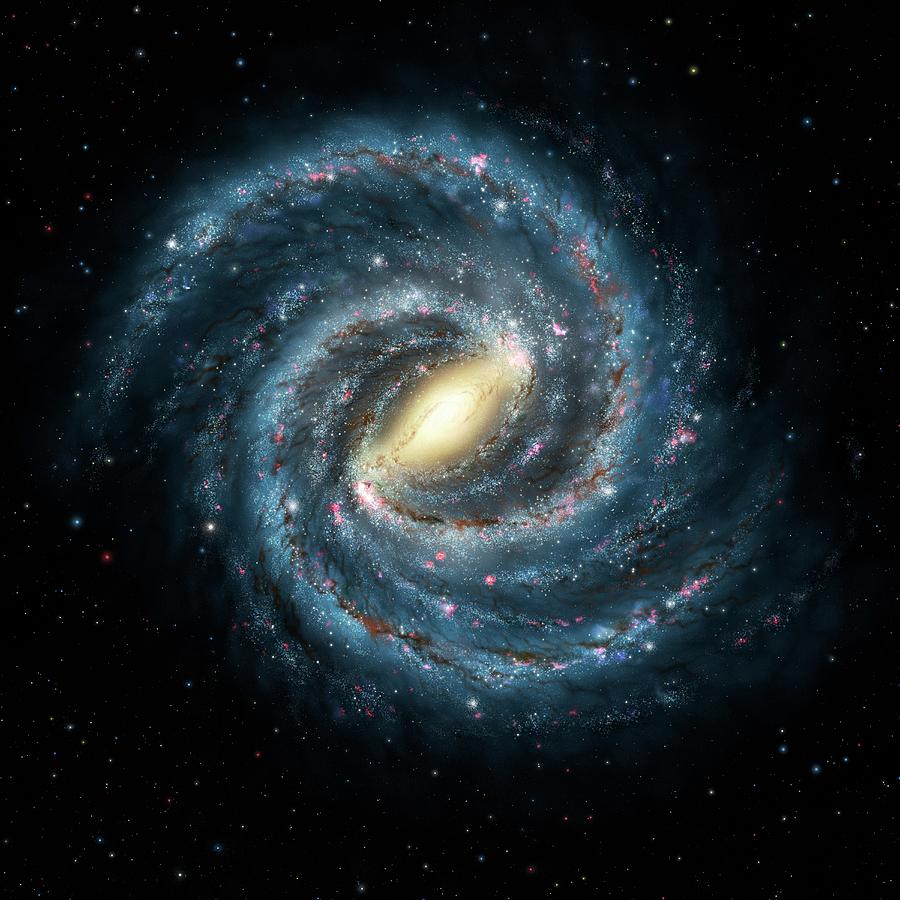
\includegraphics[width=0.25\textwidth]{images/principles}
\end{wrapfigure}

Many systems (sports, martial arts, \...) are focused around dozens or even hundreds of techniques which are thrown at a student to learn by hard, including their names, and precise definitions of what's right and what's wrong.
This is an approach which might work, but obviously has some serious disadvantages when it comes to quickly responding (picking the right technique from many within a split of a second) and more importantly the ability for individual expression.

In contrast to that, CI is centered around a few core principles, and every technique which might be taught, studied and practiced is a manifestation of those core principles.
There are therefore no real moves to be learned, but more principles to be embodied and applied in any given moment.
Once the principles are well understood, one can free oneself from the limitations of specific techniques, and questions like whether something is ``right or wrong'' can be easily answered by asking those principles.
Yet, as it is with the mastery of any art: Once the principles are fully understood, they can be broken if desired so, as: ``\textit{You can do whatever you want, as long as you know what you are doing.}''

\subsection{Grounding}\label{subsec:grounding}

With grounding we are referring to some kind of sensation (light) heaviness in the body, which makes the stance more stable, more robust and thus more connected to the ground.
Imaginary language like ``rooting'', and similar, are often used to describe this internal sensation, with its very realistic impact on the external.
This quality is the beginning of it all, without it we can't go any further, as without a firm foundation there is no house we can build upon it.
To help improving our groundedness we can use visualizations (roots growing into the ground), focusing our attention to where the sole's of the feet have contact with the floor, breathing out and relaxing the muscular tension without collapsing in one's structure, and simply thinking about words which are associated with a grounded, firm, or stable quality.

It should not be confused with stiffness, which so often lead to the illusion of groundedness, which is achieved by simply contracting all muscles; something we don't want to do as it will remove the ability to adapt in the moment, our flexibility.

\subsubsection{Small Dance}

The \gls{smalldance} is a (warming up) exercise helps the practitioner to increase one's body awareness.
It could be considered as some form of mindfulness practice, where we focus our full attention to the sensation of standing; especially of the micro movements in our ankles and whole body.
How some automatic movements, little contractions and twitches, keeping us standing upright.
Something that is beyond our consciousness, but something we can definitely tap into by being more sensitive to it.
We can use these unconscious micro movements as a source of movement by amplifying it.

It is also often used as a beginning of a grounding exercise, by shifting the weight, and keeping the center low.
Additionally to that, once the weight was totally shifted to one side, to ``double ground'' oneself to have a very clear sensation of stability and balance.

\subsection{Pouring Weight}\label{subsec:pouring-weight}

Once we have established to ``gain some weight'' by grounding, we can use that to pour it into another person's body.
The emphasis here is to slowly increase the amount of pressure where the body's have contact, instead of a quick and sudden shift, which will be difficult and fear evoking movement for your partner; ultimately even potentially dangerous.
Instead, we want to ``announce'' that there is some weight approaching, so that our partner can adjust and adapt posture and internal tension/structure to that poured weight.

\subsection{Sharing Weight}\label{subsec:sharing-weight}

The first and most important principle is trying to seek a deep connection between two bodies, sometimes also called ``\textit{umpf}''.
It is different from actively pushing with muscular force, and also different from leaning by which one shifts one's center of gravity beyond a point of no-return.
The sensation should lead to a feeling of the ground beneath the partner's feet.
The body is stable and grounded, yet its limbs and joints are soft and relaxed; like an iron stick wrapped in cotton wool.
The ultimate goal is to maintain this quality throughout (almost) all time.

\subsection{Rolling Point of Contact}\label{subsec:rolling-point-of-contact}

Instead of sliding or jumping (point of contact), by using a spiraling and rotating movement pattern, the contact (and amount of pressure) is always maintained and follows a predictable trajectory, which means both partners can anticipate the very next movement, which furthermore leads to a more ``fluid sensation'' in the dance.
For this to happen, it is required to have a more agile body, bulging out body parts and bending and flexing whenever necessary.

\subsection{Pathway Continuation}\label{subsec:pathway-continuation}

According to the physical law of inertia, and to be in accordance with it, we should never break an already moving momentum (exceptions for the master applied here).
Once spiraling in one direction it should be maintained; possibility for anticipation, predictability and therefore trust on a psychological level, but also a mere reason of energy efficiency on the physical level.

\subsection{Movement Patterns}\label{subsec:movement-patterns}

Through a heightened awareness of communication through movement, touch and sharing weight, we explore the space and the connection between through mutual physical cooperation.
Fundamental movement patterns are:

\begin{itemize}
    \item \textbf{Yielding}: softening/surrendering into incoming force or to gravity
    \item \textbf{Pushing}: expansion, taking up space
    \item \textbf{Reaching}: physically or meta-physically
    \item \textbf{Pulling}: contraction, up til collapsing
    \item \textbf{Releasing}: relaxing into what's contracted before
\end{itemize}

All of those movements can be done easily with little muscular effort if basic physical forces are acknowledged and taken advantage of, such as: gravity (falling), momentum, inertia, balancing and others.
And all of those while staying in contact.

\subsection{Relaxation}\label{subsec:relaxation}

We move usually rather relaxed; a body which is ready for action yet open for receiving tactile stimulus, open for information.
We try to achieve that by deep breathing, by keeping a fluid movement quality (``octopus quality'') and also avoid a staring eye gaze.

Yet, a relaxed state should not be confused with a collapsed one.
An active state is also not the same as a hyper-tensed one.
Within this spectrum of non-extremes, we ought to find the optimal amount of muscle tonus which is appropriate for a given situation.

\chapter{Mottos}\label{ch:mottos}

\begin{wrapfigure}{R}{0.3\textwidth}
    \centering
    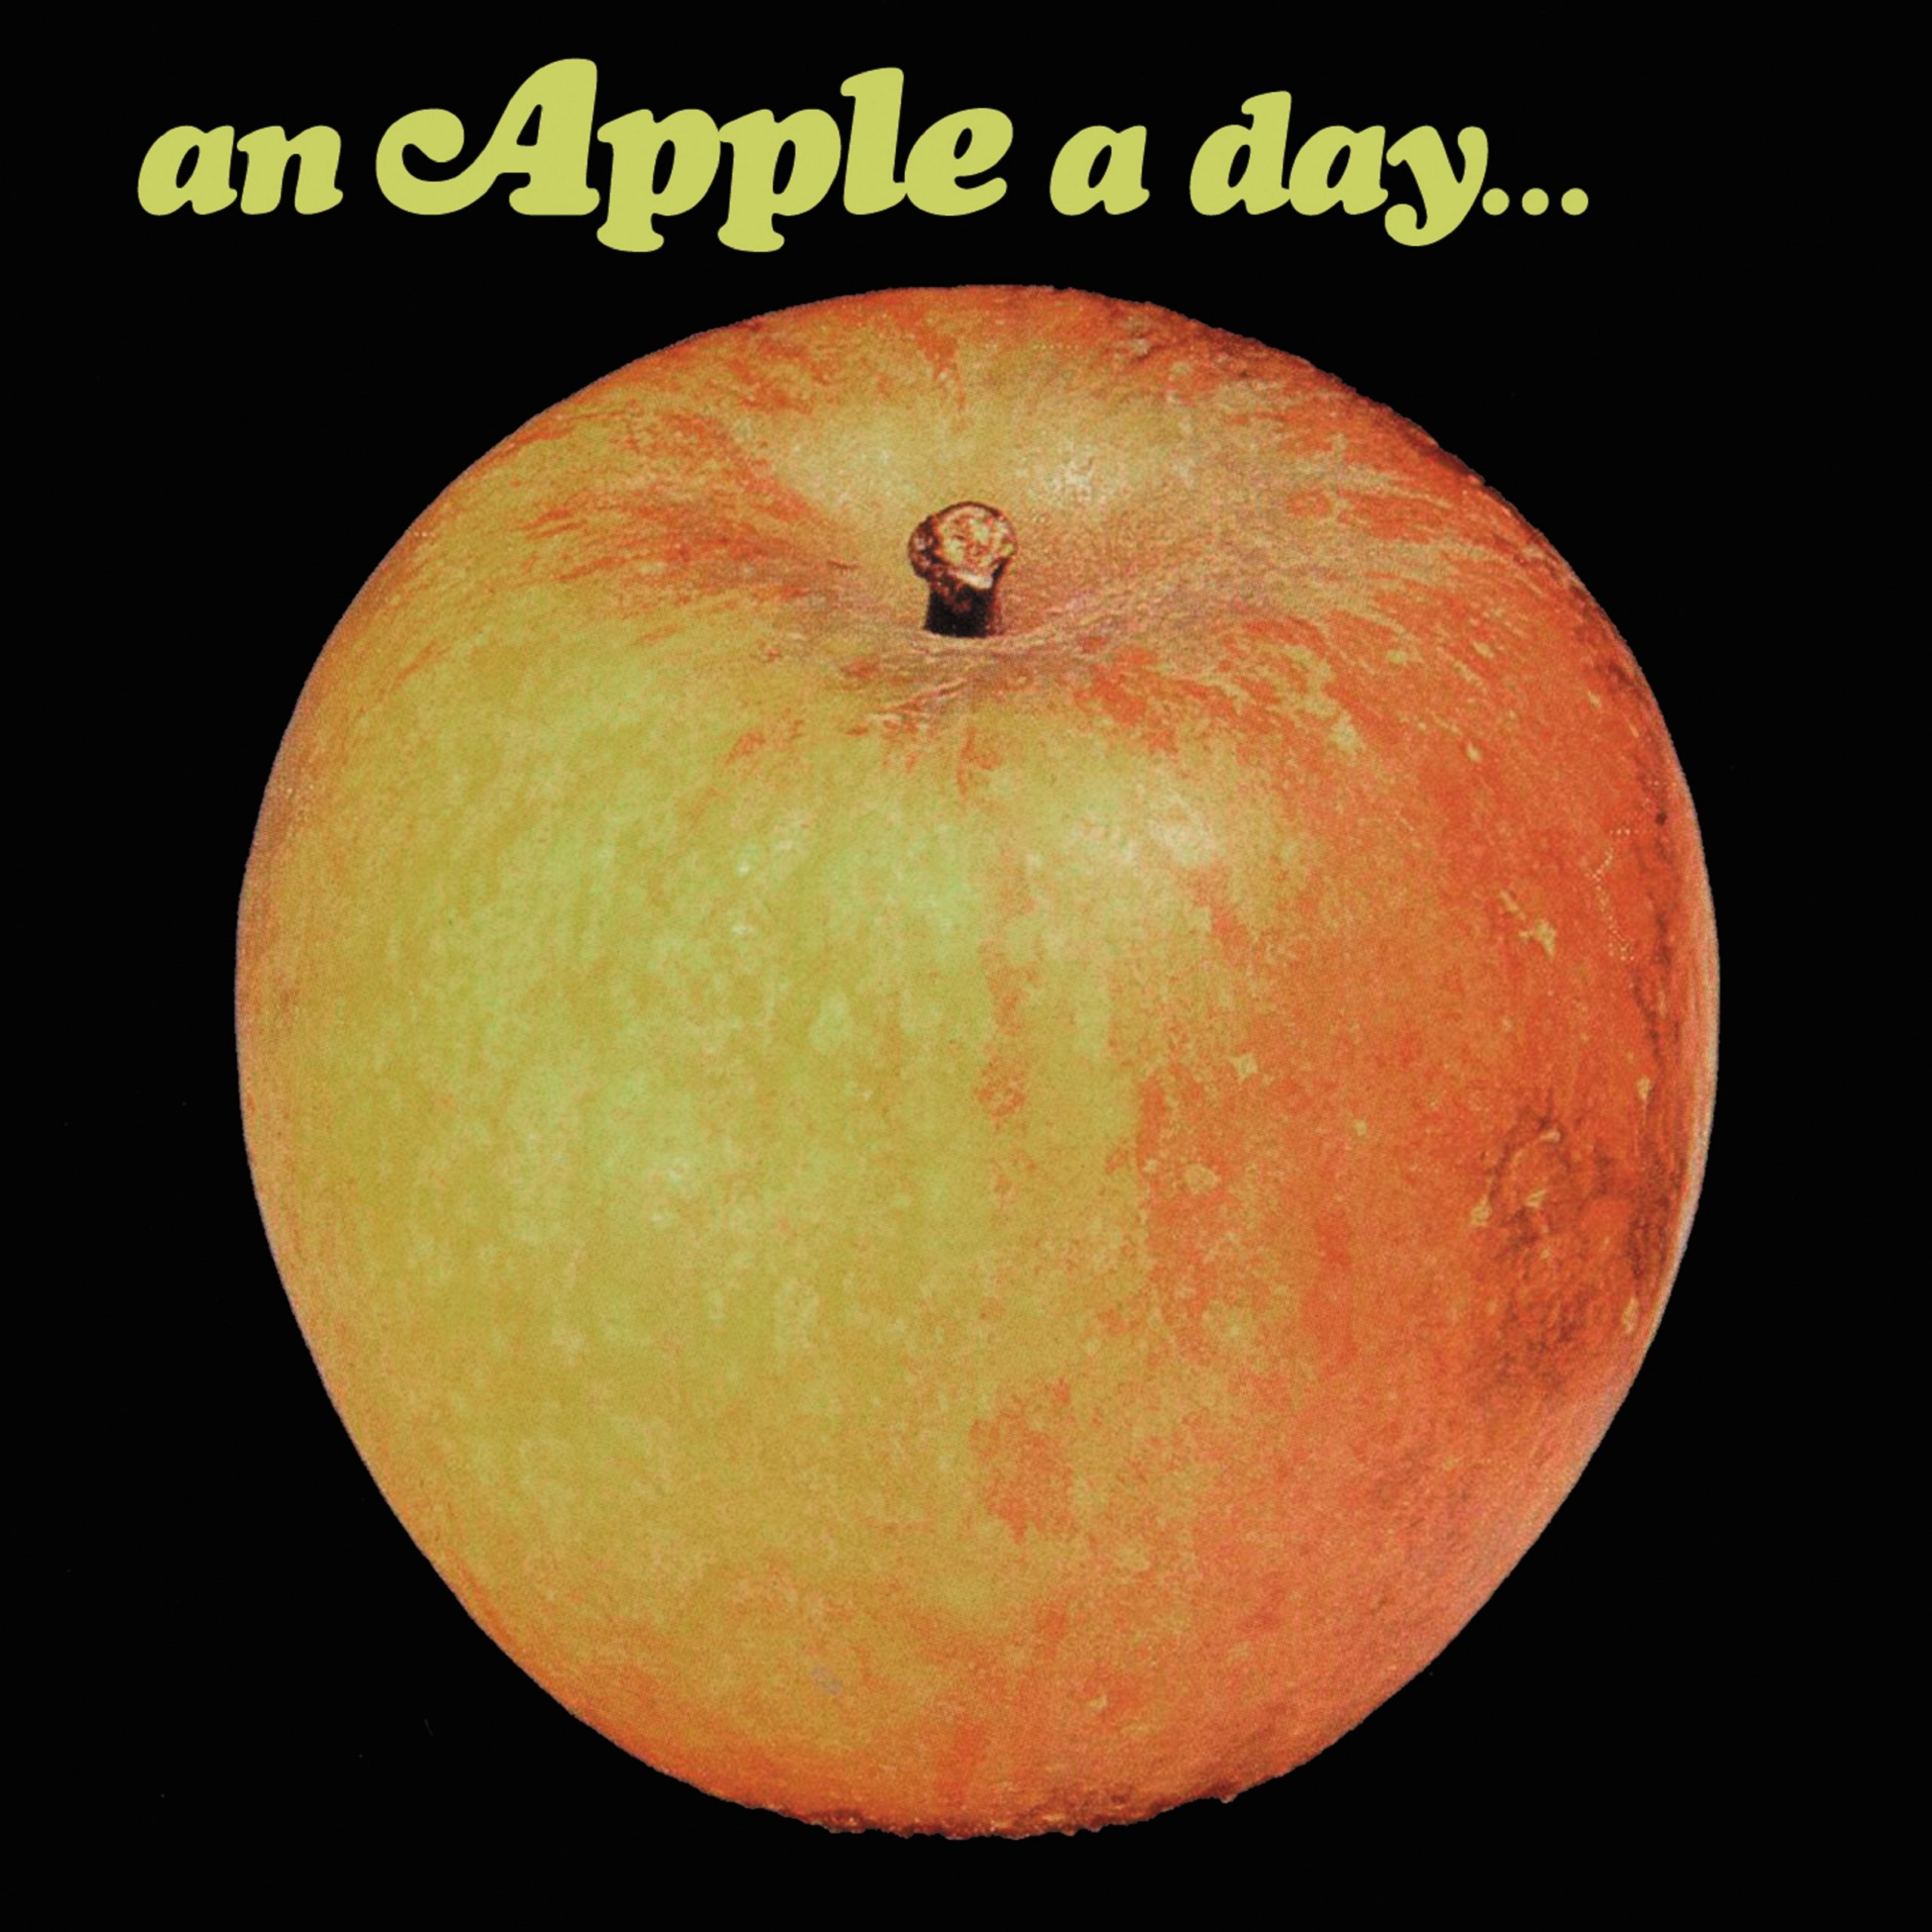
\includegraphics[width=0.25\textwidth]{images/mottos}
\end{wrapfigure}

You could also call them --universal-- guidelines, which would be semantically more specific than principles, yet not as specific as concrete techniques.
They help us improve our technique, implement the principles, and embody a quality more conforming to the core of CI\@.
They are kept short, so we can remember them quickly, and can act as part of our vocabulary.
Once we mention it to someone who is also familiar with that saying, we immediately have a common understanding within a very short period of time; something that is identical to the benefit of introducing a~\nameref{ch:jargon}.

\begin{itemize}
    \item [] \textit{Tension masks sensation.} \\
    Imagine your muscles are tensing up so much, they squeeze the nerves which then can't transmit any information anymore.
    The more \textbf{relaxed} we are, the more sensitive our skin is to touch, pressure and weight.
    Of course, we want to relax, yet not totally collapse, yet maintaining the minimum effort possible to stay stable; as little as possible, as much as necessary.
    \item [] \textit{Keep on breathing.} \\
    When getting tensed up, physically and/or emotionally, we tend to hold our breath, which is counterproductive to staying sharp, focused and relaxed.
    Instead, we continuously try to remind ourselves to breathe, and especially emphasize a deep out-breath, as the breathing out activates more our relaxation system; the parasympathetic nervous system to be precise.
    Whenever you realize that your partner becomes a bit stiff and holds his breath, it can be an effective way to non-verbally manipulate your partner into taking a big sigh as well, if you do it deliberately loud enough that he will hear it.
    It's a little bit like with the phenomena of yawning: Due to our social nature, equipped with mirror neurons, those behaviors tend to be contagious, and we can't help it but imitate it.
    \item [] \textit{We try not to fall in love with our partner, we fall in love with the dance.} \\
    Try to \textbf{depersonalize} your dance partner, seeing him as a mere physical object and by that explore the physical realm instead of the psychological, the interpersonal realm.
    It's also not a personal dance, it's a physicality; the experience is because of the practice, not because of your partner necessarily; don't attach that to a specific person, just like the teachings of Tantra tell us as well.
    Even when you had a remarkable dance with someone, once the dance is over, I'm going to say ``Thank you, and bye bye''.
    It is nevertheless possible, of course, to talk to that person later on, but please don't linger and dance the entire class or jam with that single person.
    \item [] \textit{Keep eyes open and ``wide''.} \\
    Sometimes people tend to close their eyes, or focus them constantly, fierce-fully on their partner.
    Instead, we want to keep an open gaze, perceiving everything around us, staying in connection with all the people in the room and the room itself.
    Once we start to gaze at the floor, this is usually an indication of a state of hyper-focus, which potentially closes our perception.
    Remind yourself to keep your vision leveled, stay aware and attentive.
    \item [] \textit{Dance at the edge of your level of attention, and don't cross the level of your partner's attention.} \\
    Try to \textbf{expand} what you can do regarding movement, attention, speed, techniques, and pathways.
    And also vital, listen to what your partner is able as well, and \textbf{respect} that with patience and compassion.
\end{itemize}

\section{Inspirational Mistakes}\label{sec:inspirational-mistakes}

As in general with any improvised art, mistakes are only seen as such, as soon as we declare them as being mistakes.

\begin{displayquote}
    \textit{
Imagine two improvisation actors on stage.
One says ``mouse'', the other says ``house''.
And then again, the same thing: house, then mouse.
They actually intended to go on with different rhyming words, but for whatever reason (too nervous?) they are stuck and can't come up with something new, and because they can fake it as a deliberate decision (not admitting it being a mistake, something which was not their initial desired goal; when things don't go according to a fixed plan), people in the audience might be amazed by the ``post-modern acting skills'' and interpret something into it which is actually not there.
    }
\end{displayquote}

Once you can let go of any plan, and be truly in the \textbf{present moment} with whatever is happening; once you can fully comprehend that whenever there is another person involved, any desire for control is futile \ldots then you will be able to surrender and use any happening as a source of inspiration.
Ultimately, being able to \textbf{surprise yourself}, and be fascinated by what happened to you once you let go.

\chapter{Techniques}\label{ch:techniques}

\begin{wrapfigure}{R}{0.3\textwidth}
    \centering
    
\includegraphics[width=0.25\textwidth]{images/techniques}
\end{wrapfigure}

Although CI is a \textbf{principle-based system}, meaning it doesn't have a defined set of techniques which are universally taught and practiced, there are certain reoccurring movements (``tricks'') which could be considered as techniques.
Yet, they should not be regarded as something to be followed literally, and as long as you stay within the framework of the CI principles, any adaption can be judged as correct.

\section{Technique or Principle?}\label{sec:technique-or-principle?}

The difference between technique and principle of CI is like the difference between grammar (universal and abstract) and vocabulary (specific and concrete) of language.
Even in the United States we will use the same grammar, but the words/vocabulary, and especially style/dialect will be slightly different from in the United Kingdom, Australia or anywhere else in the world; expect small hiccups to happen.
Nevertheless, we will be able to \textbf{understand} each other as the principles, the grammar stays the same.
And often it will be necessary to stay a few hours with a new teacher to embody his body language, from which the vocabulary comes.
Vocabulary, like lifts, is a rather \textbf{regional expression} of the application of the commonly shared principles.

\section{Lifts}\label{sec:lifts}

The most common -- and most impressive -- ``spice'' added to a dance are lifts.
Whenever one center is located underneath another center, a lift can be easily performed by ``pouring one's weight''\footnote{Pouring weight is one of the core principles of CI, slowly and continuously increasing the pressure, instead of jumping on our partner with a potentially heavy impact and possible injury} onto the base.

There are different kinds of lifts, but the most typical ones are hip and shoulder-lifts.
When performing a \textbf{hip-lift}, the \gls{over-dancer} usually places his butt, lower belly or side on the lower back of the \gls{under-dancer}.
The \textbf{shoulder-lift} is the highest level of a lift where one ``flies'' on the shoulder of the other person.
Those lifts are usually done standing and also while being in the ``little animal'' position, and to change for example from a hip to a shoulder-lift, the over-dancer can spiral upwards the back defying gravity.

As a base, we need to ground ourselves to become more stable (and heavy) by focusing on our \gls{centergravity},
whereas the flyer, on the other hand, tries to make himself light and engage in his \gls{centerleviathan}.

Lifting might lead to potentially dangerous situations, which require us to pay special attention to the following safety rules:

\begin{itemize*}
    \item \textbf{Not grabbing} is a general guideline, using less the hands and more the torso, yet with lifting this becomes especially important; thus no interlocking of the arms or grabbing the limbs of your flying partners.
    \item Always keep a \textbf{hollow back} (a.k.a. ``good gorilla'') to provide a stable support for your partner instead of rounding your back, which make him feel down and freak him out.
    \item Always keep your \textbf{head above ass}, otherwise your partner will most likely react with a fear response because of the danger of sliding down over your head (especially don't combine this with grabbing/interlocking).
\end{itemize*}

Read more about this in the~\nameref{ch:safety} chapter.

\section{Spirals}\label{sec:spirals}

We use a lot of spirally movement patterns in CI and pay special attention to how they are perceived, seen and anticipated in different movements in our own or someone else's body.
Moving in spirals is the perfect way to keep the pathway continuation which adds to a more enjoyable, fluid sensation during the dance.
Spiraling is considered a core movement pattern in CI and there is much more to say and experience about it.

Spirals can be very visibly be done between two body parts by moving from the distal parts of the body towards the more proximal parts.
There is a lot possible with playing with the axis, changing the axis, going within or outside the body, \ldots the limit is the imagination (and skill).
And ultimately spirals can also only by visualized, imagined, with pure intention/attention without any external visibility of movement.

\begin{exercise}
    Stand still, and have your partner touch with one of his index fingers each a point on different body parts for a second or two, and then visual and move along a connecting line between those points by using spirals around that line.
    Don't hesitate to also play with different planes to inspire new movement patterns in your partner.
\end{exercise}

\section{Negative Space}\label{sec:negative-space}

Dancing in the so-called \gls{negativespace} basically means entering, usually by reaching into it with a limb, the \gls{kinesphere} of another person without engaging in touch.
This is a common way to non-verbally invite someone for contact, to start a dance together, at a jam for example.

\section{Other Techniques}\label{sec:other-techniques}

\textbf{\Gls{body-surfing}} happens when one person rolls on the floor, and the other (usually) perpendicularly rolls over him.
Watch out if your partner is too heavy, to be able to release/distribute his weight, or simply drop your partner off in a gentle and polite way.
This usually evokes a lot of laughter due to the fun nature of it, its playfulness which reminds us of our childhood games we played.
For even more fun, consider doing a body-surf with more than two people and make some sort of ``body train''.

\textbf{Counter-balancing} is commonly used in partner-acrobatics, where the center is, for once, oppositional, instead of centers being shared.
We basically ``lean away'' from the partner, and by holding on to each other somehow, we balance each other out.

\section{Safety}\label{sec:safety}

\begin{wrapfigure}{R}{0.3\textwidth}
    \centering
    
\includegraphics[width=0.25\textwidth]{images/safety}
\end{wrapfigure}

Safety in obvious terms of ``free of injuries'' should always come first when practicing any potentially risky movement style.
Furthermore, respecting and adhering the local, specific sub-\textbf{cultural norms} which will also lead to emotional/psychological safety within the group.
Besides all these concerns about safety, it is safe to say that CI can be practiced by anyone: professionally trained dancers, recreational movers, athletes, dancers of all abilities and ages.

\subsection{Consent}\label{subsec:consent}

Consent is mainly about being able to express as well as hearing (and appropriately responding to) a ``yes'' and a ``no'', which are both possibly (and preferably) expressed non-verbally.

Of course this starts already when engaging in a dance with someone, but primarily is important when it comes to more advanced lifts.
It could be due to lack of trust into each other, fear of being lifted, considering the other person's weight as too heavy, or other reasons.
There are many elegant ways out, so that we can hold ourselves responsible for withstanding our boundaries instead of making others accountable for crossing them, ultimately ``self-dis-empowering'' ourselves.

Whenever a gentle hint by movement does not have the desired result, we can of course always cough, or lastly simply speak and be very explicit about our wishes.

\subsection{Technical Safety}\label{subsec:technical-safety}

There are many, many things which can lead to dramatic injuries, especially when being performed by non-advanced students.
Yet, for the sake of simplicity and conciseness, we will limit the list to a few, the most common ones, here:

\begin{itemize}
    \item \textbf{Head above ass}: When lifting a partner, the shoulder always by higher than the pelvis, as otherwise the person will slide down overhead.
    \item \textbf{Don't grab}: When encompassing the a partner's limb for example, that part of his body will be immovable and thus prevents him from using it as ``landing gear'' when needed, leading to a potentially severe injury.
    Additionally, it removes the agency of the other person and is considered to be simply rude in the CI scene.
    \item \textbf{Don't interlock}: When people perform a back lift and interlock the arms (and God forbid simultaneously lowering the head below the pelvis line) and they fall, the flyer might get into a state of panic and tenses up his arms, while the base will fall and not being able to use his arms, thus falling on his face with the weight of the lifted partner.
\end{itemize}

\subsection{Respectful Behavior}\label{subsec:respectful-behavior}

This will be a short list based on observations and personal experiences which seem to be worth mentioning and of course there is no claim of completeness or anything similar.

\begin{itemize}
    \item \textbf{Sensuality} is a wonderful thing, but it is not really appropriate to go into ``melting'' into your partner, falling in love, or even sexuality, and expressing this via caressing touch, cuddles and somewhat ``Tantric behavior'' during contact improvisation.
    This boundary is often crossed as the positive bonding effects of touch easily leads to more.
    At this moment it is advised to separate, to ``cool down'' and re-engage with the dance, instead of the partner.
    Caressing the skin of another person, to ``cuddle up'' and all of it is great, amazing, and please do more of it, but please refrain from doing so on the CI dancefloor.
    \item \textbf{Eye gazing} is another wonderful tool to deeply connect with another human being, yet during contact improvisation we refrain from doing so.
    We use our peripheral vision to see, and usually don't constantly dance front-to-front.
    Again: We fall in love with the dance, if with anything, and not with the partner.
    \item Speaking about \textbf{front}: It is totally fine to roll over the front side of your partner, and there is no need to avoid certain body parts (breasts, genital area).
    Once we are able to depersonalize the partner, seeing it as a physical object and letting go of the stories, there is no need to avoid certain body parts, and rather develop a more innocent and reality bound perspective.
\end{itemize}

\subsection{Etiquette}\label{subsec:etiquette}

In every subculture, there are certain norms and rules established which are not written down anywhere.
They somehow float in the minds of the people, implicitly without any mentioning.
Yet if they are broken once, there will be consequences of the group as a punishment for misbehavior.
I personally find it useful to try to capture those and make them explicit, so we can avoid unintentional misbehavior and establish as much harmony as possible.
Just know, that every scene, maybe even every group around a specific teacher, has their own set of normative rules, thus this list is just a possible set of many.

\begin{itemize}
    \item \textbf{Talking} is considered to be a distraction during contact improvisation, especially during jams.
    If loud, verbal communication is indeed needed, it can be so, there is no obligation for total silence, but be mindful whether it is truly necessary at the moment, or is it just some irrelevant chit-chat, and try to keep the volume low in order to not distract the fellow dancers.
    \item State your \textbf{name} when you dance with someone, at least at the very end, and ask for that person's name.
    It's just a nice way to acknowledge the other person and useful to furthermore possibly create a friendly bond.
    \item Proper, and appropriate, \textbf{clothing} is found in every little group, sometimes even for very rational, practical reasons.
    As such, it is recommended to wear long pants and sleeves to be able to slide on the ground; clothes which don't limit movements like jeans; button free shirts as rolling on partners with your full weight might hurt them, and also the shirt might break.
    Ultimately, we don't dress to impress but rather prefer to wear our cosy pyjamas.
    \item Although probably obvious, yet worth mentioning is \textbf{body hygiene}: Wear fresh clothes, make sure no intense bad breath, and have taken a shower before engaging in such an intimate movement form with one or more partners.
\end{itemize}

\section{Jargon}\label{sec:jargon}

\begin{wrapfigure}{R}{0.3\textwidth}
    \centering
    
\includegraphics[width=0.25\textwidth]{images/jargon}
\end{wrapfigure}

There are no universally acknowledged names for techniques, movement qualities, exercises, and so forth, but different teachers try to invent, share, and give credits to their inventions.
Over the time, an \textbf{oral tradition} has been established of passing information.
The following chapter is a rather class specific one, as the language and images developed in the area ``I grew up in'' are very local and not universal at all.
Yet, they might inspire others, or at least provide some humorist, personal benefit for you while reading it.

Introduction of a jargon, using technical, domain-specific terms, is useful to express an idea, as otherwise many, many sentences would be needed whereas instead a single word can suffice as well.
The whole purpose of introducing and using jargon is not to smart-ass, to show off one's own superiority, an act of ego arrogance, or to exclude others by using an exclusive language, but for an increased information exchange and increase in information \textbf{density and precision}.

\subsection{General}\label{subsec:general}

\begin{itemize}
    \item [] \textbf{\Gls{smalldance}} -- The subtle, unconscious micro movements of the body trying to maintain its balance.
    \item [] \textbf{\Gls{kinesphere}} -- The space which can be reached by the body/limbs without taking a step.
    \item [] \ldots \textit{for further general terms, see the glossary at the end of this book} \ldots
\end{itemize}

\subsection{Onomatopoeia}\label{subsec:onomatopoeia}

Sometimes, concepts are just way too fuzzy to be properly put into definite words.
Or there might have just no proper words yet been established, which made it necessary to develop our own few words, or even better: ``sound-terms'' (or onomatopoeia\footnote{Onomatopoeia, which has its Greek roots with the meaning of ``name-making'', which is the formation or use of words such as ``buzz'' or ``murmur'' that imitate the sounds associated with the objects or actions they refer to.}) to convey a certain meaning, quality, fuzzy principle or some abstract phenomena closer to what it meant to be:

\begin{itemize}
    \item \textbf{Botsen}: A conflict which arises when the teacher's instructions lead to a resistance based on an ``internal wisdom''; when the ``inner teacher'' and the ``outer teacher'' clash, we usually opt for the inner one and trust our gut feeling; e.g.\ Being told to jump and do a roll, but it doesn't feel safe and fear/resistance comes up, so you simply don't do it.
    (actually a Dutch word, meaning to clash, to collide; ``bot'' Dutch for bone; like two fists smashed on each other)
    \item \textbf{Hoopety Di Poop}: Techniques which look overly impressive (good to show-off), yet not necessarily showing much skill though, like jumping on each other; e.g.\ fancy technical, acrobatic stuff which usually comes with a higher risk for injury.
    \item \textbf{La La Land\footnote{Yes, ``La La Land'' is also the title of a US musical romantic comedy-drama movie from 2016 with Ryan Gosling and Emma Stone.}}: Referring to anything which is more commonly used in the area of spirituality/religion, metaphysics, esoteric, new age talk and superstitions.
    Yet, sometimes we are still using concepts from those domains nevertheless due to the lack of any other better alternatives; e.g.\ think about when talking about ``reaching beyond the physical body'', which is of course technically not possible, but it gives the right image and intention.
    \item \textbf{Mooshy Mooshy}: (or ``Muschi Muschi'') Indicating that during a dance a too sensual, and thus inappropriate atmosphere arises, with no clear intentions; ranging from simply moving very slowly caressing down to \textit{cuddle puddles} where several people like cuddling on the ground.
    This can especially often be observed when starting with dancing on the ground, often preceded by a body-scan, where things can even end up in a sort of pile of bodies (hopefully not as much as in the movie ``The Perfume'' in the end).
    \item \textbf{Oompf}: (or ``Umpf'') The preferred quality of contact between two bodies which is characterized by properly giving/sharing weight, creating a sensation of considerable amount of pressure, opposed to only slight touch; feeling each other's groundedness.
    \item \textbf{Weee}: A scream/sung sound usually expressed in moments of heightened levels of alertness/fear, to down-regulate one's own nervous system, counteracting fear/panic, and allowing the body/atmosphere to relax, release tension, and calm down; also to simply express joy at the moment about a movement, making everyone smile; e.g.\ when performing more risky lifts.
\end{itemize}

\subsection{Animals}\label{subsec:animals}

Calling things by animal names are beneficial as they have a very visual characteristic, conveying a visceral experience, because of the qualities we associate with those animal.
We mostly use their names to refer to positions, techniques and ``qualities of body''.

\begin{itemize}
    \item \textbf{Bear}: Similar to the koala, but while sitting on the ground, and the bear hugging around the torso of his partner.
    \item \textbf{Banana}: Not really an animal, but anyway a useful metaphor where the arms and legs are stretched out long, shaping the whole body like a banana; it can be practiced on the ground (a way of movement on the ground, rolling sideways and only the core touching the floor), but applied often while being on the back of a partner to spiral upwards.
    \item \textbf{Chicken Wing}: Using a ``semi lock'' with the arm pit on the partner while being lifted, or similar; often necessary if the centers are not properly stacked and becoming unbalanced.
    \item \textbf{Chicken Leg}: Same as the chicken wing but with the hip being flexed.
    \item \textbf{Crab}: The opposite of the octopus movement quality: Rigid, sharp, direct, and staccato.
    Think of the exoskeleton of the crab, when it walks sideways with its stiff limbs.
    \item \textbf{Koala}: When being lifted (or better: jumping on the partner's shoulder) hugging the upper body of the partner sideways and thus being very close to his center, while locking with your arms and legs; either around shoulders (more common) or pelvis (less common).
    It can be used as a preliminary technique for a shoulder lift.
    \item \textbf{(Little) Elephant}: Although we do like elephants, we don't like them in our studio, as their name is used to refer to steps/walking, or landing of the feet, which make a loud sound, indicating that there was no control and/or too much stiffness.
    Landing softly with no sound indicates control of movement, reversibility, precision and awareness, and also is a strong indicator for degree of safety with a partner.
    \item \textbf{Little Monkey}: As a little animal (a.k.a.: ``table-top'') but with knees lifted (a.k.a.: ``bear position'') with a light and fluent walking movement.
    Whenever we land silently, it is done so with control and elegance, which ultimately can prevent (serious) injuries.
    \item \textbf{Little Animal}: A table-top position on all fours, yet emphasizing a more dynamic, alive quality than a regular, wooden table.
    Also, when the painter is performing some movements, the little animal is actively supporting him by shaping his back accordingly, tilting and turning, flexing and extending.
    \item \textbf{Panda}: Similar to koala (and bear), but a more specific way of hugging, with belly to belly; often used while on the ground lying, keeping the centers connected all the time.
    \item \textbf{Snake}: Similar to octopus, but with a slightly different image to connect differently; having lots of movements in hands and spine.
    \item \textbf{Octopus}: A movement quality which indicates aliveness/relaxation in all joints/body parts, each of them being controlled by their own intelligence; fluid, soft and smooth; opposite of the crab.
\end{itemize}

\section{Anatomy}\label{sec:anatomy}

\begin{wrapfigure}{R}{0.3\textwidth}
    \centering
    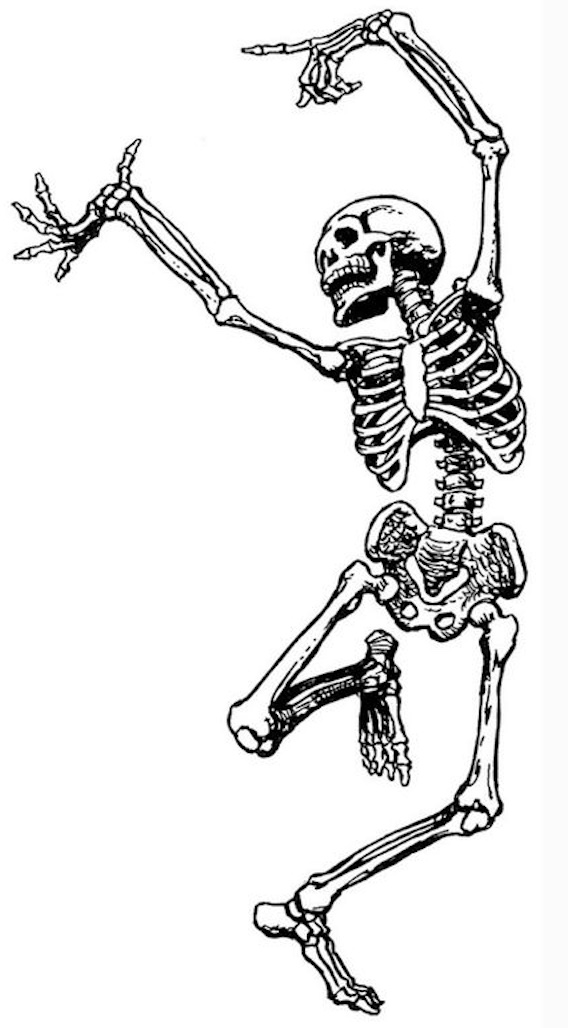
\includegraphics[width=0.25\textwidth]{images/anatomy}
\end{wrapfigure}

As with every practice dealing with the human body, a basic \textbf{understanding} of the anatomy is mandatory, adding a tremendous benefit for the practitioner-student and also gets handy with \textbf{communication}.
The field of anatomy is huge, and it doesn't need to be studied in-depth of course.
Making yourself familiar with a few, important medical terms and the basic concepts of the human body, to also have a theoretical understanding of what's happening during the dance while enable you to see things in a broader context.

\subsection{Terminology}\label{subsec:terminology}

The wording used in anatomy/medicine is built from sub-elements (which usually originated from Latin), thus:
Learning first the elements, and then putting them together to be able to infer the meaning of more complex, compound terms.

\subsubsection{Orientation}

Because a person can stand, sit, lie, or be in all kind of positions, it is necessary to have an absolute frame of reference to provide orientation instructions.
What someone means with using simple language of ``up'' or ``front'' is often not clear, thus these following words lead to a more \textbf{non-ambiguous language}.

\begin{itemize*}
    \item \textbf{anterior/posterior} = front/back
    \item \textbf{ventral/dorsal} = front/back of the torso
    \item \textbf{superior/inferior} = above/below
    \item \textbf{cranial/caudal} = head-/tail-wards
    \item \textbf{proximal/distal} = towards to/away from center
    \item \textbf{medial/lateral} = towards/away the midline
    \item \textbf{superficial/profound} = more outside/inside the body
\end{itemize*}

\subsubsection{Movements}

Each body part can move in certain ways and directions based on the type of joint (see below) and how muscles pull on it.
Again, instructing someone to ``move up'' is ambiguous, whereas ``flex the right knee'' is clear as it can be.

\begin{itemize*}
    \item \textbf{extension/flexion} = making the angle of a joint bigger / smaller (or: stretch/bend)
    \item \textbf{internal/external (medial/lateral) rotation} = arm / leg rotating in the shoulder/hip-joint; counter-/clockwise towards to/away from the body
    \item \textbf{adduction/abduction} = moving towards or away the body / midline
    \item \textbf{elevation/depression} = moving (shoulder) superior / inferior direction
    \item \textbf{pronation/supination} = rotating forearm so that palm facing up/down
    \item \textbf{dorsi-/plantar-flexion} = move the ankle towards the dorsum (superior surface, up) or plantar (sole, down) also often called ``point''
    \item \textbf{in-/eversion} = move the sole towards, inwards / away the median plane, inwards
    \item \textbf{opposition/reposition} = thumb and little finger together / spread
    \item \textbf{pro-/retraction} = anterolateral / posteromedial movement of the scapula (move shoulder forward/backward)
    \item \textbf{circumduction} = conical (not really circular) movement of a limb extending from the joint its moved by
\end{itemize*}

If we take for example a simple shoulder roll, it can be dissected in four movements: elevation, retraction, depression, and protraction.
Or similar with drawing circles with the toes, moving the ankle: dorsi-flexion, eversion, plantar-flexion, and inversion.

Terms derived from lateral movement include:

\begin{itemize*}
    \item \textbf{Uni-lateral} = ``unus'' meaning ``one'', on one side of the body
    \item \textbf{Bi-lateral} = ``bis'' meaning ``twice'', on both sides of the body
    \item \textbf{Homo-(Ipsi-)lateral} = ``ipse'' meaning ``same''
    \item \textbf{Contra-lateral} = ``contra'' meaning ``against'', e.g. arm on one side, and leg on the other side, creating a diagonal, like we do while walking; also one hemisphere of the brain is controlling the other side of the body
\end{itemize*}

Sometimes the Latin word for left (``sinister'') and right (``dexter'') are being used instead.
Check the next time you have a medical report available, like an X-ray, and you will see these terms pop up; consider yourself a nerd from now on.

\subsection{Structures}\label{subsec:structures}

Next to being familiar with the very basic words of positions and directions, we need also to be able to refer concrete structures (bones and muscles) which can be located in relation to each other and moved in a specific way.
Make yourself thus familiar with some (by far not all) anatomical terms which help you further understand this medical jargon.

\subsubsection{Bones}

The human body consists of \textbf{206 bones} (usually); yet by birth we have a few more which results to 280.
The head and trunk (the axial skeleton) make up 80 bones and the limbs (the appendicular skeleton) the other 126.
There are 27 bones for each hand (19 for phalanges plus metacarpals, and 8 carpals), and 26 for each foot (phalanges, metatarsals, and tarsals).

\begin{itemize*}
    \item \textbf{atlas and axis} = two top most cervical vertebrae (top part of the spine)
    \item \textbf{clavicle} = the collar bone
    \item \textbf{coccyx} = the tailbone (last part of the spine)
    \item \textbf{cranium} = the skull (cervical = neck)
    \item \textbf{patella} = the knee cap
    \item \textbf{processus} = a bony thing bulging out, usually for tendons to attach to
    \item \textbf{ribs} = true ribs (1-7, sternum connection), false ribs (8-10/12, cartilage), and floating ribs (11-12, no connection)
    \item \textbf{scapula} = the shoulder blade
    \item \textbf{sacrum} = big triangular bone at the base of the spine
    \item \textbf{SIAS} = Spina Illiaca Anterior Superior (front top pointy bone structure of the pelvis)
    \item \textbf{spina} = the spine, consisting of 33 vertebrae: 7 cervical, 12 thoracic, 5 lumbar, 5 fused sacrum, 4 fused coccyx
    \item \textbf{sternum} = the chest bone
\end{itemize*}

\subsubsection{Muscles}

There are \textbf{between 600 and 840 muscles} within the typical human body, depending on how they are counted (and some mutations).

\begin{itemize*}
    \item \textbf{abs} = abdominal muscles with 3 layers wrapped around the belly
    \item \textbf{core muscles} = basically everything attached to the spine
    \item \textbf{diaphragm} = muscle for breathing at the bottom of the ribs
    \item \textbf{glutes} = buttocks consisting of gluteus maximus, medius, and minimus
    \item \textbf{obliques} = part of the core, at the sides of the abs
    \item \textbf{pectoralis} = the chest muscle (major and minor)
    \item \textbf{pelvic floor} = similar to diaphragm but at the bottom of the torso
    \item ``\textbf{stomach muscles}'' = the stomach is an organ, which indeed has (involuntary) muscles, but it's located on the left side underneath the ribs, and should not be confused with the abs / lower belly!
    \item \textbf{trapezius} = at top shoulder around the neck
    \item \textbf{transverse} = part of the core, like a belt around it
\end{itemize*}

\subsection{Planes}\label{subsec:planes}

\begin{wrapfigure}{R}{0.3\textwidth}
    \centering
    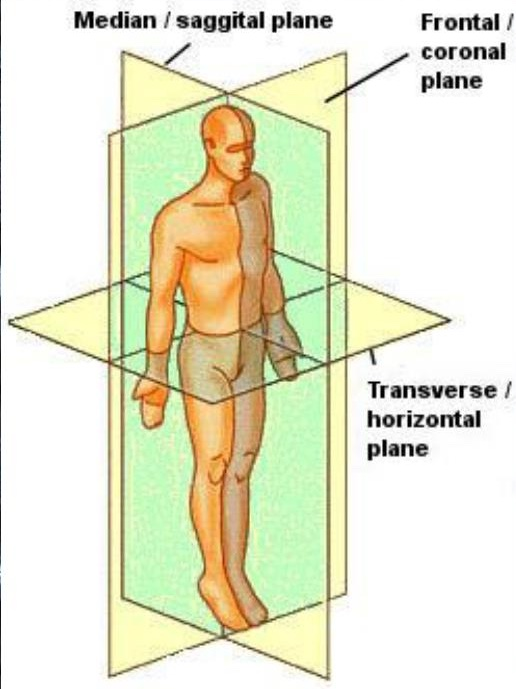
\includegraphics[width=0.25\textwidth]{images/anatomy_planes}
    \caption{The three anatomic \textbf{planes} for the human body.}
\end{wrapfigure}

We differentiate 3 different anatomical planes in which movement can happen:

\begin{enumerate}
    \item \textbf{Frontal Plane}: Also called \textit{Coronal Plane} or \textit{Vertical Plane} and, not surprisingly, represents the plane when looking from the front of the body, dividing the body in an anterior/posterior part.
    The directions can be medial/lateral thus resulting in the movements of: ad-/abduction, elevation/depression and in-/eversion.
    \item \textbf{Sagittal Plane}: Also called \textit{Lateral Plane}, \textit{Longitudinal Plane} or \textit{Anteroposterior Plane}, which is going through the midline and shows the body when looking from the side, separating it into a left/right part.
    The directions are thus anterior/posterior and movements are flexion/extension and pro-/retraction.
    \item \textbf{Transverse Plane}: Also called \textit{Axial Plane}, \textit{Horizontal Plane} (the other two planes are vertical) or \textit{Cross-Sectional Plane}, and divides the body into a top/bottom part.
    Directions are thus superior/inferior and allowing movements like rotation, supination/pronation and circumduction.
\end{enumerate}

\subsection{Joints}\label{subsec:joints}

Bones are connected through joints where muscles (together with tendons) can evoke movement.
For different movements, \textbf{different types} of (synovial) joints are needed:

\begin{itemize*}
    \item \textbf{Ball/Socket}: free movement; e.g. hip, shoulder
    \item \textbf{Pivot}: rotation; head (atlantoaxial), elbow (radioulnar)
    \item \textbf{Hinge}: flexion/extension; elbow (humeroulnar), knee
    \item \textbf{Saddle}: fingers-hand (trapeziometacarpal)
    \item \textbf{Condyloid}: fingers/wrist (metacarpophalangeal)
    \item \textbf{Plane}: hand (intercarpal) and feet (tarsal)
    \item \textbf{Gliding}: mini bones in feet
\end{itemize*}

\section{Physics}\label{sec:physics}

\begin{wrapfigure}{R}{0.3\textwidth}
    \centering
    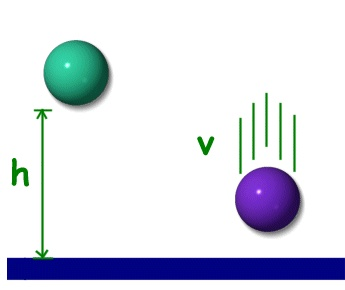
\includegraphics[width=0.25\textwidth]{images/physics}
\end{wrapfigure}

Physics is a huge and fascinating science, dealing with the big (astronomy, astrophysics), the small (nuclear and particle physics), the universal (electromagnetism, thermodynamics) and the more complicated (quantum physics, relativity); basically how the universe behaves, or at least how matter moves through space and time as well as energy and force.
For our purpose though, we will focus on mechanics and its sub-branches, the fundamental concepts of time, space and how they give rise to higher phenomena encountered during CI\@.
Preferably after that chapter you are familiar with common terms such as: gravity, vector, inertia, force, momentum, kinetics.

\subsection{Energy}\label{subsec:energy}

The word ``energy'' is just too often misused in the spiritual world as some metaphysical, psycho-telepathic mystery.
In physics, we define it simply as ``the capacity for doing work'', and as such different forms exist: potential (position), kinetic (movement), thermal (heat), nuclear (atom), electrical (charges), chemical, and so on.
All forms of energy are associated with motion: Any given body has kinetic energy if it's in motion.
A tensioned device such as a bow, a spring, or your tendons, though at rest, have the potential for creating motion; it contains potential energy.
Energy can neither be created nor destroyed, but only transformed from one form to another (principle stated in the first law of thermodynamics).

\subsection{Mechanics}\label{subsec:mechanics}

Here we are interested in the relationship between force, matter and motion, as seen from a Newtonian perspective, focusing on motion (\textbf{kinematics} or ``the geometry of motion'') and forces (\textbf{dynamics}).

Newton's laws of motion (classical mechanics):

\begin{enumerate}
    \item ``\textit{A body remains at rest, or in motion at a constant speed in a straight line, except insofar as it is acted upon by a force.}'' \\
    This law expresses the principle of \textbf{\gls{inertia}}: the natural behavior of a body is to move in a straight line at constant speed. \\
    A body's motion preserves the status quo, but external forces can disturb this.
    \item ``\textit{The net force on a body is equal to the body's instantaneous acceleration multiplied by its instantaneous mass or, equivalently, the rate at which the body's momentum changes with time.}'' \\
    This law is about motion, or as we call it nowadays \textbf{\gls{momentum}}. \\
    It depends upon the amount of matter contained in a body, the speed at which that body is moving, and the direction in which it is moving. \\
    In modern notation, the momentum of a body is the product of its mass and its velocity. \\
    The forces acting on a body add as \textbf{\gls{vector}s} (quantities with both magnitutde and direction), and so the total force on a body depends upon both the magnitudes and the directions of the individual forces. \\
    When the net force on a body is equal to zero, then by Newton's second law, the body does not accelerate, and it is said to be in \textbf{mechanical equilibrium}.
    \item ``\textit{To every action, there is always opposed an equal reaction; or, the mutual actions of two bodies upon each other are always equal, and directed to contrary parts.}'' \\
    This relates to the conservation of momentum.
\end{enumerate}

Further candidates for additional laws could be:
\begin{enumerate}
    \item \textit{Uniformly accelerated motion}, also known as: free fall, when a body falls (in the absence of air resistance), it will accelerate at a constant rate. \\
    The speed with which it falls is proportional to the elapsed time, and the acceleration is the same for all bodies, independent of their mass (law of universal gravitation).
    \item \textit{Uniform circular motion}, which contains the centripetal force (required to sustain the acceleration towards the center). \\
    The centrifugal force is, on the other hand, an inertial (fictitious/pseudo) force that is directed radially away from the axis of rotation.
    \item \textit{Harmonic motion}, as shown by a spring-mass system or a pendulum.
\end{enumerate}

\subsection{Relation to CI}\label{subsec:relation-to-ci}

We constantly encounter those concepts during practicing CI: When our bodies, as physical objects, are in motion, they have a certain momentum, which they want to keep (inertia) until a force is acted upon them.
Gravity pulls us downwards, and we can use levers to take advantage of it, without having the need to exert lots of muscular force, wasting our energy and making the practice effortful, instead of effortless.
Keeping track of the trajectory of moving objects helps us to keep a continuous pathway, making the movements more smooth, and less edgy/clumsy, but also more predictable for our partner, thus resulting in an increased level of trust.

\chapter{Movement}\label{ch:movement}

\begin{wrapfigure}{R}{0.3\textwidth}
    \centering
    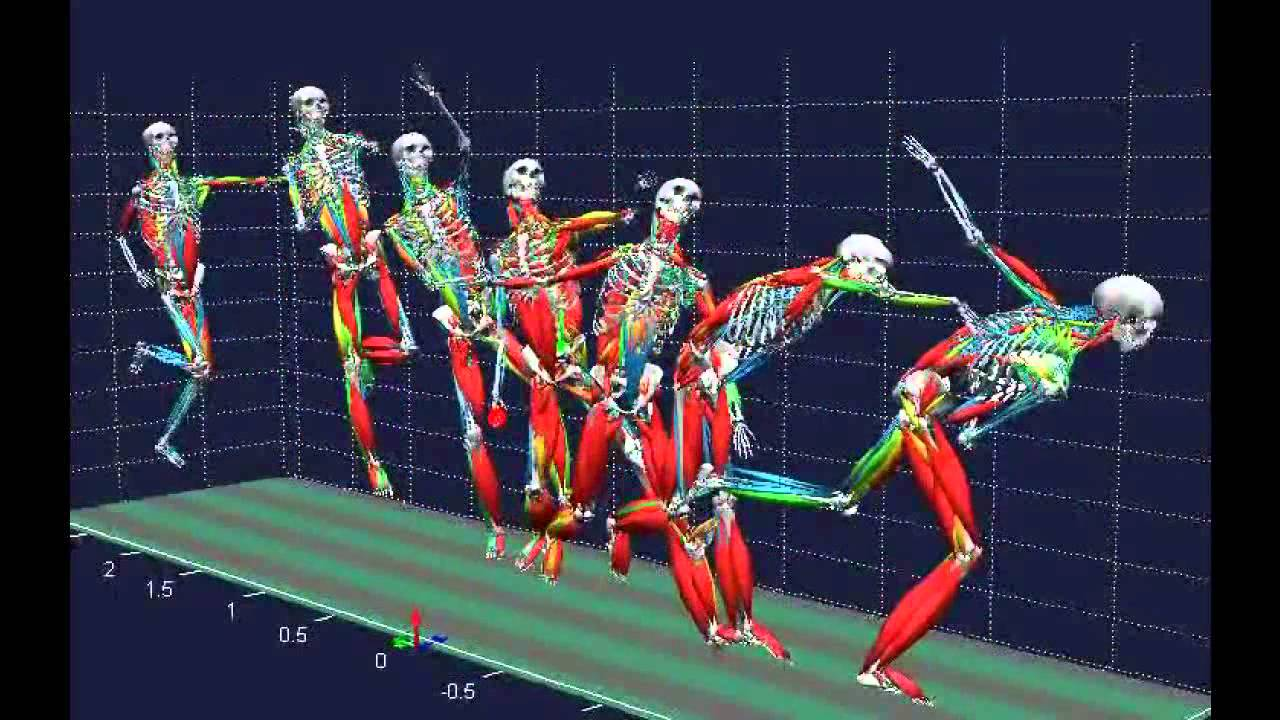
\includegraphics[width=0.25\textwidth]{images/movement}
\end{wrapfigure}

This chapter is based on the previous ones about anatomy/physics, and how these concepts give raise to higher concepts we encounter while practicing CI\@.
We will take a look at the fascinating science of movement, movement theory and a bit of biomechanics, and also deal with more abstract views on movement as maybe known from the dancing world.
For more experienced (improvisation) dancers, a lot of the things mentioned here might sound familiar, for the more inexperienced among us this can open a totally new perspective on movement.

\section{Movement Qualities}\label{sec:movement-qualities}

There are different imagined \textbf{dimensions} we can play with, to tap into different qualities on how to use our body, giving it a different flavor, allowing us to do different techniques, and by knowing the pros and cons of each quality, we can apply them in the right moment to elevate our technical skill and also keep things safe for ourselves and our partner.

\begin{itemize}
    \item [] \textbf{Muscle Tone} \\
    We can play a lot with tone, which is the amount of tension we create in our muscles that makes us either more relaxed or more stiff.
    In general, we prefer to maintain the least amount of effort, a minimum muscle tension; as little as possible, as much as necessary.
    By being more relaxed, we are more flexible, can adapt to an ever-changing situation, and also are more receptive via our tactile sense, being able to receive more information, to listen better.
    To have some images to play with, think of moving through air (well, you don't have to imagine that, as we constantly do that --duh).
    Instead, think of you being a cloud, floating through the sky (sure, that's better, we usually never do that one).
    Now increase tension by imagining moving through water, how it creates a small but continuous resistance, preventing you from sharp, edgy movements, from breaking a fluent pathway.
    The next increase in resistance could be achieved by imagining something like honey, sticky and slowing down your movements, having you to add more muscle effort.
    And as a final step, imagine being stuck in concrete, which maybe has not yet fully harden, still making you almost unmovable.

    \item [] \textbf{Speed} \\
    Moving on to the very obvious dimension of slowness and fastness.
    The slow can be extremely slow, to gain lots of information of internal sensations.
    The fast can be released in an explosive manner, like a shockwave through the whole body.
    Both, and everything in-between, can be alternated rapidly, to gain more control (of speed).

    \item [] \textbf{Kinesphere} \\
    The degree of extension of the limbs into the space --without stepping-- is called \gls{kinesphere} with which we can play with.
    We could segregate it into a small (body), medium (elbows, knees), large (wrists, ankles) and extra large (fingers, toes), and something more abstract going even beyond (projecting outwards), the universe.
    Each of them is creating a differently sized ball, or more like an egg shape, around us in which we are limited to move within and also want to stay in constant contact with.

    \item [] \textbf{Levels} \\
    Next to extension into space, we can, of course, take different levels in vertical space: Up (standing), middle (hinged, or on hands and knees being a ``little animal'') and floor work (lying on the ground).
    With the help of relaxation and tension, we can quickly change our position on the vertical axis and play with explosive dynamics.
    Also, mirroring your dance partner, staying at a different (not the same as with imitating) level then he, can be an challenging, fun, and engaging expierence to explore.

    \item [] \textbf{Isolation} \\
    The isolation of certain body parts can also be fun --and challenging at the same time-- to play with.
    The most simple one is to divide the body into upper and lower, left and right side, same side or cross side (homo- or contra-lateral, see the anatomy section for explanation of terminology), or move only in a certain plane.

    \item [] \textbf{Shapes} \\
    The forms we are drawing in air can be another dimension.
    Think of straight lines (edgy, staccato) versus roundness (flowy, fluid, air).
    People who have experience with the practice of 5 Rhythms might be familiar with those concepts and make use of them.
\end{itemize}

To bring those qualities to a next level, try to \textbf{combine} them in different ways.
Often slow, fluid and soft go together, but how about changing one of them to the other extreme?!
Or the legs are in the large kinesphere being soft and staccato, while the arms in the small kinesphere and hard and fluid.
Have a partner telling you what parts should be in which quality, to surprise yourself by finding combinations you would not have thought of alone.

\section{Partner Dance}\label{sec:partner-dance}

\textit{Disclaimer}: There is lots to tell about dancing with one (or more) partner(s), and this subsection will be far from mentioning all the most relevant there is, but ought to give just a quick glimpse of what might be encountered at the beginning of your CI journey.

Humans are \textbf{social animals}, and as such we have countless neuronal networks dedicated to processing social information, hardwired bonding tendencies leading to the ability to read each other, get in-tuned with each other, ultimately leading to harmony in groups.
Think of basic empathy, which is associated to mirror neurons in our brain, which for example leads us to yawn once we see someone else yawning, or feel the pain we observe in that funny (?) video clip where someone falls from a skateboard.
If we want to feel how someone else is feeling, we might simply want to put our full presence with that person (or even a group) and feel inside our bodies of what's happening; there is a high chance that what we experience is the other person's state of being.
Using a more ``flowery language'', we could say that this is the ability of ``\textit{feel the other person's energy}'' --whatever is supposed to be meant by (mis-)using the word ``energy'' here.

As human beings we also have the innate need to \textbf{be seen} by others; being ignored as one of the worst punishments we can experience, leading to feelings of isolation, exclusion and loneliness.
The biggest present therefore we can give each other is to \textbf{mirror} each other's movements; explicitly acknowledging the other person's existence, putting one's attention to that person, copying his movements, which is also called ``\textit{kinesthetic resonance}''.
Of course counter-mirroring has the same effect (you go down, I go up; you go left, I go right), as it still maintains a form of connection we can play with.

\section{Body Awareness}\label{sec:body-awareness}

Let's have a look of how we actually become aware of our bodies.
The biological and physiological base of how this fascinating organic machinery --roughly-- works.

\subsection{Vestibular System}\label{subsec:vestibular-system}

This is our sense of \textbf{balance} and spatial orientation for the purpose of movement coordination, and is all well known to us.
It consists of two components: The (three, as there are three dimensions) \textit{semicircular canals} for rotational movements, and the \textit{otoliths} for linear accelerations.
Signals from those are sent to the muscles to keep us upright and control posture, allowing us to maintain our desired position in space.
Together with our proprioception, we can understand our body's dynamics and kinematics in any given moment.

\subsection{Proprioception}\label{subsec:proprioception}

\Gls{proprioception} allows us --as a sort of 6th sense, the ``kinesthetic sense''-- to be consciously aware of movement, force and body \textbf{position}.
It tells us our body's position in the space, that is the relative positioning of neighboring body parts, and the strength of effort needed for movement.
Try for example to close your eyes and touch your nose; you will be able to do this without looking (in a mirror, or in complete darkness) because of little cells (little \textit{spindles} which are spring-like protein molecules which are stretched inside your muscles) in your body being aware of the \textbf{amount of stretch} they experience (joint position sense), which is then processed subconsciously by your brain giving raise to a bodily sensation.
Everyone is familiar with the knee-jerk reflex, where the patellar tendon is rapidly stretched to an extreme (usually with the help of a hammer), which leads to an immediate response (a reflex) to counteract that and protect the tissue from injury.

Related sensations are \textit{exteroception}, the perception of the outside world, and \textit{interoception}, the perception of internal sensations like pain and hunger.

\subsection{Kinesthesia}\label{subsec:kinesthesia}

\Gls{kinesthesia} is the awareness of position and \textbf{movement} of body parts using sensory organs (proprioceptors, mechanosensory neurons) in muscles, tendons and joints.
It's crucial in muscle memory and hand-eye coordination.
Sometimes it's confused with proprioception, but those two are different concepts.
If you have an inner ear infection for example, and the sense of balance is affected, this would degrade the proprioceptive, but not the kinesthetic sense.
Moreover, proprioception is more about joint position (more subconscious cognitive awareness of your body in space and balance) whereas kinesthesia is more about awareness of joint movement (more conscious body's motion, behavioral).

\subsection{Neuronal Processing}\label{subsec:neuronal-processing}

\textbf{Neuromuscular control} is the efferent (signal from the central nervous system to the body) response to an afferent (sensory) input, which is the functional component to movement and athletic activities that is referred to as dynamic stability.
Sensory input comes as (different types of\footnote{The four mechanoreceptors are: Meissner corpuscle for heavy pressure, Pacinian corpuscle for vibraiton, Merkel disks for light touch and Ruffini endings for skin stretch}) \textbf{mechanoreceptors} located in muscles, capsules and ligaments, allowing us awareness of joint position, movement, and acceleration.

All that information (vestibular, proprioceptive, kinesthetic) including the visual input is sent to the brain, where it is processed and integrated to allow us to create an overall representation of body position, movement and acceleration.

\section{Space Harmony}\label{sec:space-harmony}

This movement theory --and practice, also called \textit{Choreutics}-- was developed by the Austrian-Hungarian dancer and choreographer Rudolf Laban, to study the natural sequences of movements we follow in daily life; studying ``the art of movement'' to recognize spatial patterns.

When dancing, the term \textbf{\gls{kinesphere}} is used to refer to the space immediately reachable by your limbs without changing your place on the ground.
We can use up a lot of that space within this sphere (\textit{Far Reach Kinesphere}), just a bit (\textit{Near Reach Kinesphere}) or something in-between (\textit{Mid Reach Kinesphere}).

\begin{wrapfigure}{R}{0.3\textwidth}
    \centering
    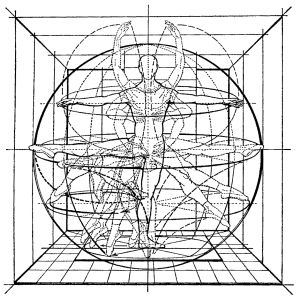
\includegraphics[width=0.25\textwidth]{images/kinsphere}
    \caption{The \textbf{kinesphere} around the body reachable by extended limbs.}
\end{wrapfigure}

Furthermore, Mister Laban believed that there are three types of movers which prefer different \textbf{levels}: Those who enjoy leaping and springing off the ground move in \textit{High Level}, those with more sensuous movement enjoying the \textit{Central (Middle) Level}, and those who prefer more earth-bound movements who stayed in the \textit{Deep (Low) Level}.

Within the kinesphere we can move from one point to another through different approaches, so-called \textbf{pathways}: When movement is initiated from (or passes through) the body's center we take the \textit{Central Pathway}, along the outer limits of the kinesphere it takes a \textit{Peripheral Pathway}, and when the movement passes between center and periphery it takes a \textit{Transverse Pathway}.

There is of course much more to say about this, including the Laban Movement Analysis (LMA) which is a method and language for describing, visualizing, interpreting, and documenting movement, but this would go beyond the purpose of this book.

\chapter{Resources}\label{ch:resources}

The content of this book might not have been enough for your mental thirst for information and insight, in which case the following collection of further resources will hopefully leave you with greater satisfaction.

\section{Practice}\label{sec:practice}

In case you are looking to practice (classes, workshops, festivals) anywhere in the world, check out the \href{https://ciglobalcalendar.net}{CI global calendar}, and if you need something more local (in the Netherlands) lookup the community calendar \href{https://amsterdamjam.nl}{amsterdamjam.nl} or go directly to \href{https://tomgoldhand.com}{Tom Goldhand's website}.

\section{Books}\label{sec:books}

There are about 10 good books written which are specifically about CI\@.

\begin{itemize}
    \setlength\itemsep{0em}
    \item ``\href{https://www.amazon.com/Sharing-Dance-Improvisation-Directions-Anthropological/dp/0299124444}{Sharing the Dance: Contact Improvisation and American Culture}'' by Cynthia J. Novack (A good book about the history of the form, origins and stories)
    \item ``\href{https://www.amazon.com/Caught-Falling-Confluence-Contact-Improvisation/dp/0937645095}{Caught Falling: The Confluence of Contact Improvisation}'' by Nancy Stark Smith
    \item ``\href{https://www.amazon.com/Contact-Improvisation-Introduction-Vitalizing-Dance/dp/0786426470}{Contact Improvisation: An Introduction to a Vitalizing Dance Form}'' by Cheryl Pallant
    \item ``\href{https://www.amazon.com/Contact-Improvisation-Dancing-Interaction-Introduction/dp/1841261386}{Contact Improvisation: Moving, Dancing, Interaction}'' by Thomas Kaltenbrunner
    \item ``\href{https://www.amazon.com/Improvisation-Body-Mind-Centering-Teaching-Learning/dp/0976044900}{Contact Improvisation and Body-Mind Centering: A Manual for Teaching and Learning Movement}'' by Annie Brook
    \item ``\href{https://www.amazon.com/Taken-Surprise-Dance-Improvisation-Reader/dp/0819566489}{Taken by Surprise: A Dance Improvisation Reader}'' by Ann Cooper Albright and David Gere
    \item ``\href{https://www.amazon.com/Dancing-Deeper-Still-Practice-Improvisation/dp/1775243044}{Dancing Deeper Still: The Practice of Contact Improvisation}'' by Martin Keogh
    \item ``\href{https://contredanse.org/en/product/gravity/}{Gravity}'' by Steve Paxton
\end{itemize}

\section{Videos}\label{sec:videos}

It's good practice to watch ``the classics'' (everything between 1972 and 1980) once in a while.

\begin{itemize}
    \setlength\itemsep{0em}
    \item ``\href{https://www.youtube.com/watch?v=9FeSDsmIeHA}{The invention of CI}'' - The very early beginnings, 1972
    \item ``\href{https://www.youtube.com/watch?v=5gEfVJBhwrQ}{Magnesium}'' - The actual piece from that research is called magnesium, 1972
    \item ``\href{https://www.youtube.com/watch?v=xKlO-2e3gHo}{Chute}'' - A few years later, 1979
    \item ``\href{https://www.youtube.com/watch?v=k768K\_OTePM}{Fall After Newton}'' - Many things have changed here, 1987, originally 22 minutes long
    \item \href{https://www.youtube.com/@contactquarterly}{contactquarterly channel} - A YouTube channel containing some videos of the early beginnings (e.g. Chute, Magnesium, Peripheral Vision, Soft Pallet)
    \item ``\href{https://www.youtube.com/watch?v=hlIRjfto7o0}{Life Lessons Learned Through Contact Improvisation}'' - An interesting TEDx video-clip to see the connection of CI to general life
    \item ``\href{https://www.youtube.com/watch?v=n1D9RU2GbBo}{Gogolfest 2016 Contact Improvisation}'' - Simply inspiring to watch
    \item \href{https://www.youtube.com/watch?v=H8JiB2Nv5Qo}{A couple of basic exercises} - Something to practice by yourself as a beginner
    \item \href{https://www.youtube.com/watch?v=_82Od5NM4LI}{Steve Paxton Talking Dance} - The creator of CI giving an almost 2 hours talk about dancing, 2015
\end{itemize}

\section{Websites}\label{sec:websites}

\begin{itemize}
    \setlength\itemsep{0em}
    \item \url{https://contactquarterly.com} (CQ Unbound Journal, the main platform and official channel for the global CI community)
    \item \url{https://www.materialforthespine.com/} - Steve Paxton's work and research after he passed on CI and researched walking and material for the spine
    \item \url{https://nancystarksmith.com/underscore/} - A long-form dance improvisation structure/notation using graphical symbols.
    \item \url{http://ecite.org} (European Contact Improvisation Teachers Exchange)
    \item \url{https://contactimprov.com}
    \item \url{https://contactimprovblog.com}
    \item \url{https://bodyresearch.org/contact-improvisation}
    \item \url{https://www.dancemagazine.com/rules-of-contact-improv-class/}
    \item \url{https://joerghassmann.com/other-themes/what-is-contact-improvisation/}
    \item \url{https://dancespirit.com/contact-improv/}
    \item \url{https://en.wikipedia.org/wiki/Contact_improvisation}
\end{itemize}


%\listoffigures
%\listoftables
\printglossaries

\end{document}
